
\documentclass{IOS-Book-Article}

\usepackage{mathptmx}
\usepackage{rotating,todonotes, xspace}
\usepackage{amssymb}
\usepackage[section]{placeins}
\usepackage{makeidx}  % allows for indexgeneration
\usepackage{algorithm}
\usepackage{algpseudocode}
\usepackage{graphicx}
\usepackage{float}
\usepackage{subcaption}
\captionsetup{compatibility=false}
\usepackage{wrapfig}
\usepackage{array}
\usepackage{multicol}
\usepackage{amsmath}
\usepackage{amssymb }
\usepackage{bm}
\usepackage{float}
%\usepackage{times}
%\normalfont
%\usepackage[T1]{fontenc}
%\usepackage[mtplusscr,mtbold]{mathtime}
%
\begin{document}
\begin{frontmatter}              % The preamble begins here.

%\pretitle{Pretitle}
\title{Fault Tolerance and Task Clustering\\
 in Scientific Workflows}
\runningtitle{Fault Tolerant Clustering}
%\subtitle{Subtitle}

\author[A]{{Weiwei} {Chen}%
\thanks{Corresponding Author: Weiwei Chen, University of Southern California, Information Sciences Institute, Marina del Rey, CA, USA; E-mail:
weiweichen@acm.org.}},
\author[A]{Rafael Ferreira de Silva}, 
\author[A]{{Ewa Deelman}}
and 
\author[B]{{Thomas} {Fahringer}}

\runningauthor{W. Chen et al.}
\address[A]{University of Southern California, Information Sciences Institute, Marina del Rey, CA, USA}
\address[B]{University of Innsbruck, Institute for Computer Science, Innsbruck, Austria}

\begin{abstract}
Large scale scientific workflows can be composed of many fine computational granularity tasks. Task clustering has been proven to be an effective method to reduce execution overhead and increase the computational granularity of workflow tasks executing on distributed resources. However, a job composed of multiple tasks may have a greater risk of suffering from failures than a job composed of a single task. Our theoretic analysis and simulation results demonstrate that transient failures can have a significant impact on the runtime performance of scientific workflows that use existing clustering policies that ignore failures. We aim to optimize the workflow makespan by adjusting the clustering granularity in the presence of failures. We propose a general task failure modeling framework and use a Maximum Likelihood Estimation based parameter estimation process to address these performance issues. We further propose three methods to improve the runtime performance of executing workflows in faulty environments. A trace based simulation is performed and it shows that our methods improve the workflow makespan significantly for five important applications.    
\end{abstract}

\begin{keyword}
scientific workflows\sep fault tolerance\sep parameter estimation\sep failure\sep machine learning \sep clustering
\end{keyword}
\end{frontmatter}

\thispagestyle{empty}
\pagestyle{empty}

\section*{Introduction}


Scientific workflows can be composed of many fine computational granularity tasks and the runtime of these tasks may be even shorter than the system overhead. System overhead is the period time during which miscellaneous work other than the user’s computation is performed. Task clustering \cite{Chen2013a, Singh2008, Chen2012, Maheshwari2012, Ferreira-granularity-2013, Integration2012} is a technique that merges several short tasks into a single job such that the job runtime is increased and the overall system overhead is decreased. However, existing clustering strategies ignore or underestimate the impact of the occurrence of failures on system behavior, despite the current and increasing importance of failures in large-scale distributed systems, such as Grids \cite{Bresnahan2011, Deelman2004, Rubing2005}, Clouds \cite{Deelman2008, Berriman2010, Bresnahan2011} and dedicated clusters. Many researchers \cite{Zhang2004, Tang1990, Schroeder2006, Sahoo2004} have emphasized the importance of fault tolerance design and indicated that the failure rates in modern distributed systems are significant. Among all possible failures, we focus on transient failures because they are expected to be more prevalent than permanent failures \cite{Zhang2004}. For example, denser integration of semiconductor circuits and lower operating voltage levels may increase the likelihood of bit-flips when circuits are bombarded by cosmic rays and other particles \cite{Zhang2004}. 

In task clustering, a clustered job consists of multiple tasks. A task is marked as failed (task failure) if it is terminated by unexpected events during the computation of this task. If a task within a job fails, this job has a job failure, even though other tasks within this job do not necessarily fail. 
In a faulty environment, there are several options for reducing the influence of workflow failures. First, one can simply retry the entire job when its computation is not successful as in the Pegasus \cite{Deelman2004}, ASKALON \cite{fahringer2007askalon} and Chemomentum \cite{schuller2008chemomentum}. However, some of the tasks within the job may have completed successfully and it could be a waste of time and resources to retry all of the tasks. Second, the application process can be periodically checkpointed such that when a failure occurs, the amount of work to be retried is limited. However, the overheads of checkpointing can limit its benefits \cite{Zhang2004}. Third, tasks can be replicated to different nodes to avoid failures that are related to one specific worker node \cite{Plankensteiner2009}. However, inappropriate clustering (and replication) parameters may cause severe performance degradation if they create long-running clustered jobs. As we will show, a long-running job that consists of many tasks has a higher job failure rate even when the inter-arrival time of failures is long. 

In this paper, we assume a task-level monitoring service is available. A task-level monitor tells which tasks in a clustered job fail or succeed, while a job-level monitor only tells whether this job fail or not. The job-level fault tolerant clustering has been discussed in our prior work \cite{Chen2012}. 

We propose two horizontal methods and one vertical methods to improve the existing clustering techniques in a faulty environment. The first horizontal method retries the failed tasks within a job. The second horizontal solution dynamically \emph{adjusts the granularity or clustering size} (number of tasks in a job) according to the estimated inter-arrival time of task failures. The vertical method reduces the clustering size by half in each job retry. 
%We further analyze the runtime performance of combining horizontal methods and vertical methods in different ways. 

In this paper we view the sequence of failure events as a stochastic process and study the distribution of its inter-arrival times, i.e. the time between failures. Our work is based on an assumption that the the distribution parameter of the inter-arrival time is a function of the \emph{type of task}. Tasks of the same type have the same computational program (executable file). In the five workflows we examine in this paper, tasks at the same horizontal level (defined as the longest distance from the entry task of the workflow) of the workflows has the same type. 
The characteristics of tasks such as the task runtime, memory peak and disk usage are highly related to the task type \cite{da2013toward, Juve2013}.
Task type related failure is a type of failure that only occurs to some specific types of tasks. Samak \cite{Samak2011} et al. have analyzed 1,329 real workflow executions across six distinct applications and concluded that the type of a task is among the most significant factors that impacted failures. 

%A node failure only occurs to some specific execution nodes. 
Compared to our prior work in \cite{Chen2012}, we add a parameter learning process to estimate the distribution of the task runtime, the system overhead and the inter-arrival time of failures. We adopt an approach of prior and posterior knowledge based Maximum Likelihood Estimation (MLE) that has been recently used in machine learning. Prior knowledge about the parameters are modeled as a distribution with known parameters. Posterior knowledge about the execution information are also modeled a distribution with a known \emph{shape parameter} and an unknown \emph{scale parameter}. The shape parameter affects the shape of a distribution and the scale parameter affects the stretching or shrinking of a distribution. Both parameters control the characteristics of a distribution. The distribution of the prior and the posterior are in the same family if the likelihood distribution follows some specific distribution and they are called \emph{conjugate distributions}. For example, if the likelihood is a Weibull distribution and we model prior knowledge as an Inverse-Gamma distribution, then the posterior is also an Inverse-Gamma distribution. This simplifies the estimation of parameters and integrates the prior knowledge and posterior knowledge gracefully. More specifically, we define the parameter learning process with only prior knowledge as the static estimation. The process with both prior knowledge and posterior knowledge is called the dynamic estimation since we update the MLE based on the information collected during the execution.  

The two horizontal methods were introduced and evaluated in \cite{Chen2012} on two workflows. In this paper, we complement this previous paper by studying (\emph{i}) the performance gain of using two horizontal methods and one vertical method over a baseline execution on a larger set of workflows (five widely used scientific applications); (\emph{ii}) the performance impact of the variance of the distribution of the task runtime, the system overheads and the inter-arrival time of failures; (\emph{iii}) the performance difference of dynamic estimation and static estimation with variation of inter-arrival time of failures.  

The rest of this paper is organized as follows. Section \ref{sec:related} gives an overview of the related work. Section \ref{sec:models} presents our workflow and failure models. Section \ref{sec:clustering} details our fault tolerant clustering methods. Section \ref{sec:experiments} reports experiments and results, and the paper closes with a discussion and conclusions. 



\section{RELATED WORK}
\label{sec:related}

Failure analysis and modeling \cite{Tang1990} presents system characteristics such as error and failure distribution and hazard rates. Schroeder et al. \cite{Schroeder2006} has studied the statistics of the data, including the root cause of failures, the mean time between failures, and the mean time to repair. Sahoo et al. \cite{Sahoo2004} analyzed the empirical and statistical properties of system errors and failures from a network of heterogeneous servers running a diverse workload. Oppenheimer et al. \cite{Oppenheimer2002} analyzed the causes of failures from three large-scale Internet services and the effectiveness of various techniques for preventing and mitigating service failure. McConnel \cite{McConnel} analyzed the transient errors in computer systems and showed that transient errors follow a Weibull distribution. In \cite{Sun2003, Iosup2008} Weibull distribution is one of the best fit for the workflow traces they used.  Based on these work, we measure the inter-arrival time of failures in a workflow and then provide methods to improve task clustering.  

More and more workflow management systems are taking fault tolerance into consideration. The Pegasus workflow management system \cite{Deelman2004} has incorporated a task-level monitoring system and used job retry to address the issue of task failures. They also used provenance data to track the failure records and analyzed the causes of failures \cite{Samak2011}. Plankensteiner et. al. \cite{plankensteiner2009fault} have surveyed the fault detection, prevention and recovery techniques in current grid workflow management systems such as ASKALON \cite{fahringer2007askalon}, Chemomentum \cite{schuller2008chemomentum}, Escogitare \cite{laforenza2007biological} and Triana \cite{taylor2007triana}. Recovery techniques such as replication, checkpointing, task resubmission  and task migration etc. have been provided. In our paper, we are specifically joining the work of failure analysis and the optimization in task clustering. To be best of our knowledge, none of existing workflow management systems have provided such features. 

Overhead analysis~\cite{Ostberg2011, Prodan2008} is a topic of great interest in the Grid community. Stratan et al.~\cite{Stratan2008} evaluate in a real-world environment Grid workflow engines including DAGMan/Condor and Karajan/Globus. Their methodology focuses on five system characteristics: overhead, raw performance, stability, scalability, and reliability. They pointed out that head node consumption should not be negligible and the main bottleneck in a busy system is often the head node. Prodan et al.~\cite{Prodan2008} offered a complete Grid workflow overhead classification and a systematic measurement of overheads. In Chen et al.~\cite{Chen2011}, we extended~\cite{Prodan2008} by providing a measurement of major overheads imposed by workflow management systems and execution environments and analyzed how existing optimization techniques improve runtime by reducing or overlapping overheads. The prevalent existence of system overheads is an important reason why task clustering provides significant performance improvement for workflow-based applications. In this work, we aim to further improve the performance of task clustering in a faulty environment. 

Machine learning has been used to predict execution time \cite{Rubing2009, 1015660, 1542747, da2013toward} and system overheads~\cite{Chen2011}, and develop probability distributions for transient failure characteristics. Duan et.al. \cite{Rubing2009} used Bayesian network to model and predict workflow task runtimes. The important attributes (such as the external load, arguments etc. ) are dynamically selected by the Bayesian network and fed into a radial basis function neural network to make further predictions. Ferreira da Silva et. al. \cite{da2013toward} used regression trees to dynamically estimate task behavior including process I/O, runtime, memory peak and disk usage. In our paper, we reuse the knowledge gained from prior work on failure analysis, overhead analysis and task runtime analysis. We then use prior knowledge based Maximum Likelihood Estimation to integrate both the knowledge and runtime feedbacks and adjust the estimation accordingly. 

The low performance of \emph{fine-grained} tasks is a common problem in widely distributed platforms where the scheduling overhead and queuing times at resources are high, such as Grid and Cloud systems. Several works have addressed the control of task granularity of bag of tasks. For instance, Muthuvelu et al.~\cite{Muthuvelu2005} proposed a clustering algorithm that groups bag of tasks based on their runtime---tasks are grouped up to the resource capacity. Later, they extended their work~\cite{4493929} to determine task granularity based on task file size, CPU time, and resource constraints. Recently, they proposed an online scheduling algorithm~\cite{Muthuvelu2010} that groups tasks based on resource network utilization, user's budget, and application deadline. Ng et al.~\cite{Keat2006} and Ang et al.~\cite{Ang2009} introduced bandwidth in the scheduling framework to enhance the performance of task scheduling. Longer tasks are assigned to resources with better bandwidth. Liu and Liao~\cite{Liu2009} proposed an adaptive fine-grained job scheduling algorithm to group fine-grained tasks according to processing capacity and bandwidth of the current available resources. Although these techniques significantly reduce the impact of scheduling and queuing time overhead, they did not consider fault tolerance.

Task granularity control has also been addressed in scientific workflows. For instance, Singh et al.~\cite{Singh2008} proposed a level- and label-based clustering. In level-based clustering, tasks at the same level can be clustered together. The number of clusters or tasks per cluster are specified by the user. In the label-based clustering, the user labels tasks that should be clustered together. Although their work considers data dependencies between workflow levels, it is done manually by the users, which is prone to errors. Recently, Ferreira da Silva et al.~\cite{Ferreira-granularity-2013} proposed task grouping and ungrouping algorithms to control workflow task granularity in a non-clairvoyant and online context, where none or few characteristics about the application or resources are known in advance. Their work significantly reduced scheduling and queuing time overheads, but did not consider fault tolerance.





\section{Design and Models}
\label{sec:models}



\subsection{Workflow Model}


\label{sec:model}


A workflow is modeled as a directed acyclic graph (DAG), where each node in the DAG often represents a workflow task ($t$), and the edges represent dependencies between the tasks that constrain the order in which tasks are executed. \emph{Dependencies} typically represent data-flow dependencies in the application, where the output files produced by one task are used as inputs of another task. Each \emph{task} is a computational program and a set of parameters that need to be executed. 
%Figure~\ref{fig:model_odag} (left) shows an illustration of a DAG composed of four tasks. 
This model fits several workflow management systems such as Pegasus~\cite{Deelman2004}, Askalon~\cite{fahringer2007askalon}, and Taverna~\cite{Oinn2004}. 

In this paper, we assume there is only one execution site with multiple compute resources, such as virtual machines on the clouds. 
Figure~\ref{fig:model_system} shows a typical workflow execution environment that targets a homogeneous computer cluster, for example, a dedicated cluster or a virtual cluster on Clouds. The submit host prepares a workflow for execution (clustering, mapping, etc.), and worker nodes, at an execution site, execute jobs individually. The main components are introduced below:

\begin{figure}[!htb]
\centering
  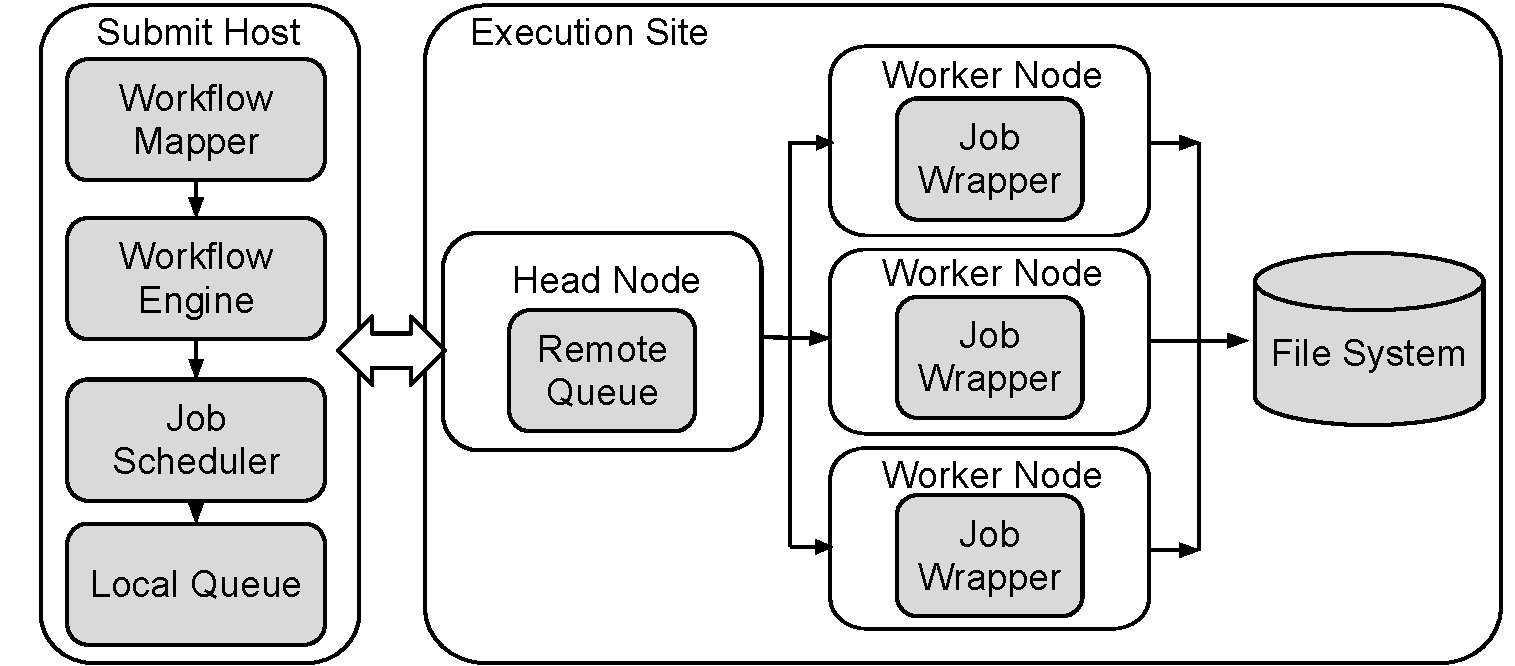
\includegraphics[width=0.95\linewidth]{model.pdf}
  \caption{A workflow system model.}
  \label{fig:model_system}
\end{figure}

\paragraph{Workflow Mapper} Generates an executable workflow based on an abstract workflow~\cite{Deelman2004} provided by the user or a workflow composition system. It also restructures the workflow to optimize performance and adds tasks for data management and provenance information generation. In this work, the workflow mapper is used to merge small tasks together into a job such that system overheads are reduced (\textbf{task clustering}). A job is a single execution unit in the workflow execution systems and is composed of one or more tasks. 

\paragraph{Workflow Engine} Executes jobs defined by the workflow in order of their dependencies. Only jobs that have all their parent jobs completed are submitted to the Job Scheduler. The Workflow Engine relies on the resources (compute, storage, and network) defined in the executable workflow to perform computations. The elapsed time from when a job is released (all of its parents have completed successfully) to when it is submitted to the job scheduler is denoted as the workflow engine delay. %The workflow engine delay is usually configured by users to assure that the entire workflow scheduling and execution system is not overloaded. 

\paragraph{Job Scheduler and Local Queue} Manage individual workflow jobs and supervise their execution on local and remote resources. The elapsed time from when a task is submitted to the job scheduler to when it starts its execution in a worker node is denoted as the queue delay. It reflects both the efficiency of the job scheduler and the resource availability. 

\paragraph{Job Wrapper} Extracts tasks from clustered jobs and executes them at the worker nodes. The clustering delay is the  elapsed time of the extraction process.

\begin{figure}[!htb]
	\centering
	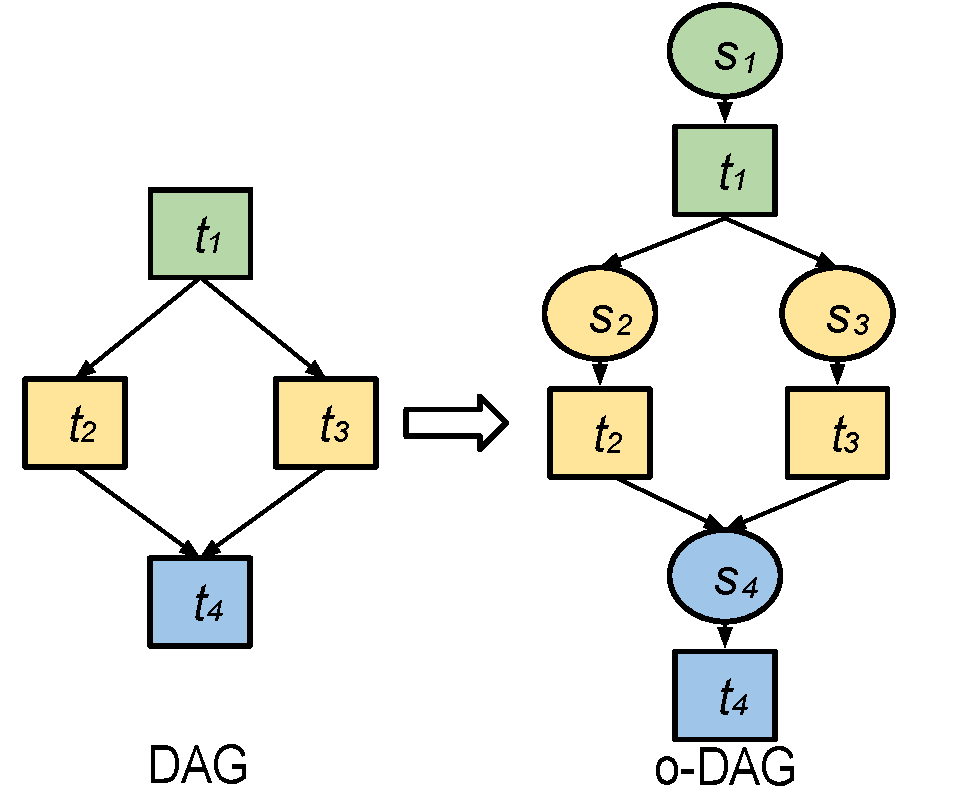
\includegraphics[width=0.6\linewidth]{odag.pdf}
	\captionof{figure}{Extending DAG to o-DAG. `s' denotes a system overhead. }
	\label{fig:model_odag}
\end{figure}

We extend the DAG model to be overhead aware (o-DAG). System overheads play an important role in workflow execution and constitute a major part of the overall runtime when tasks are poorly clustered~\cite{Chen2011}. Figure~\ref{fig:model_odag} shows how we augment a DAG to be an o-DAG with the capability to represent system overheads ($s$) such as workflow engine and queue delays. In addition, system overheads also include data transfer delay caused by staging-in and staging-out data. This classification of system overheads is based on our prior study on workflow analysis~\cite{Chen2011}. 

With an o-DAG model, we can explicitly express the process of task clustering. In this paper, we address task clustering horizontally and vertically. \textbf{Horizontal Clustering} (HC) merges multiple tasks that are at the same horizontal level of the workflow, in which the horizontal level of a task is defined as the longest distance from the entry task of the DAG to this task. \textbf{Vertical Clustering} (VC) merges tasks within a pipeline of the workflow. Tasks at the same pipeline share a single-parent-single-child relationship, which means a task $t_a$ is the unique parent of a task $t_b$, which is the unique child of $t_a$. 

Figure~\ref{fig:model_hc} shows a simple example of how to perform HC, in which two tasks $t_2$ and $t_3$, without a data dependency between them, are merged into a clustered job $j_1$. A job $j$ is a single execution unit composed by one or multiple task(s). Job wrappers are commonly used to execute clustered jobs, but they add an overhead denoted by the clustering delay $c$. The clustering delay measures the difference between the sum of the actual task runtimes and the job runtime seen by the job scheduler. 
After horizontal clustering, $t_2$ and $t_3$ in $j_1$ can be executed in sequence or in parallel, if parallelism in one compute node is supported. In this work, we consider sequential executions only. Given a single resource, the overall runtime for the workflow in Figure~\ref{fig:model_hc} (left) is $runtime_l= \sum_{i=1}^{4}(s_i+t_i)$, and the overall runtime for the clustered workflow in Figure~\ref{fig:model_hc} (right) is $runtime_r=s_1+t_1+s_2+c_1+t_2+t_3+s_4+t_4$.  $runtime_l > runtime_r$ as long as $c_1 < s_3$, which is the case in many distributed systems since the clustering delay within a single execution node is usually shorter than the scheduling overhead across different execution nodes. 

\begin{figure}[!htb]
\centering
 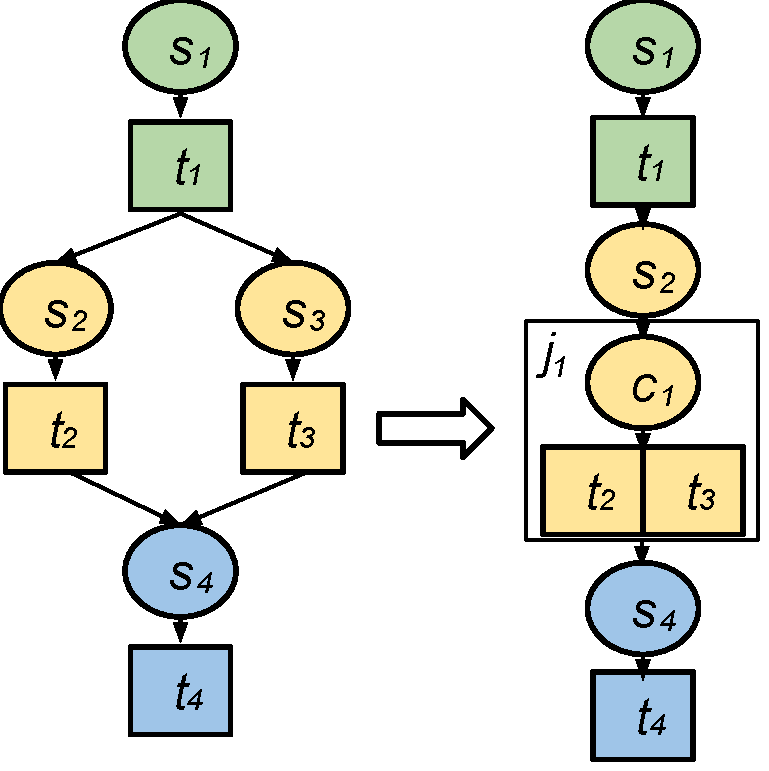
\includegraphics[width=0.45\linewidth]{hc.pdf}
  \captionof{figure}{An example of horizontal clustering (color indicates the horizontal level of a task).}
  \label{fig:model_hc}
\end{figure}

\begin{figure}[!htb]
\centering
 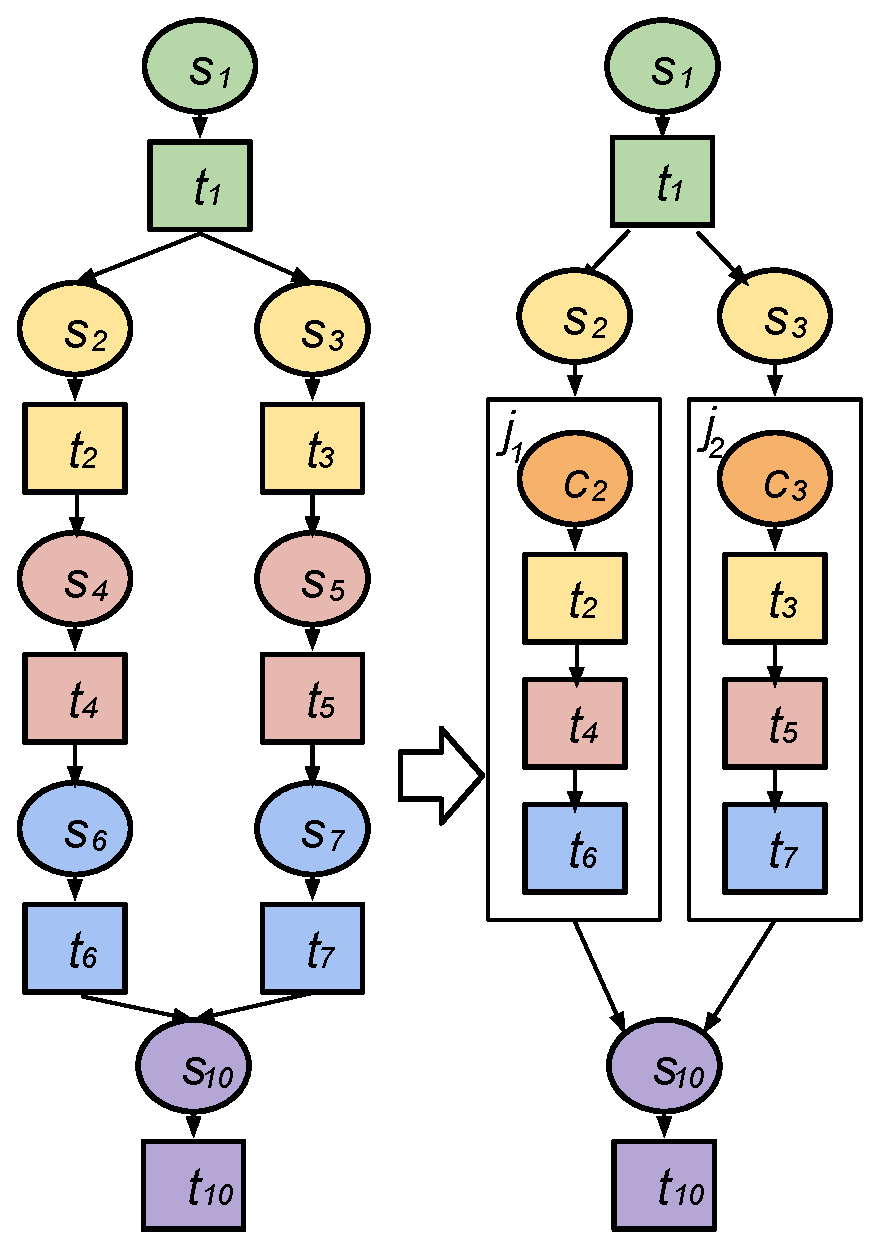
\includegraphics[width=0.5\linewidth]{vc.pdf}
  \captionof{figure}{An example of vertical clustering.}
  \label{fig:model_vc}
\end{figure}

Figure~\ref{fig:model_vc} illustrates an example of vertical clustering, in which tasks $t_2$, $t_4$, and $t_6$ are merged into $j_1$, while tasks $t_3$, $t_5$, and $t_7$ are merged into $j_2$. Similarly, clustering delays $c_2$ and $c_3$ are added to $j_1$ and $j_2$ respectively, but system overheads $s_4$, $s_5$, $s_6$, and $s_7$ are removed. 

In this paper, the \emph{goal} is to reduce the workflow makespan in a faulty environment by adjusting the clustering size ($k$). In task clustering, the clustering size ($k$) is an important parameter to influence the performance. We define it as the number of tasks in a clustered job. For example, the $k$ in Figure~\ref{fig:model_hc} is 2. The reason why task clustering can help improve the performance is that it can reduce the scheduling cycles that workflow tasks go through since the number of jobs has decreased. The result is a reduction in the scheduling overhead and possibly other overheads as well \cite{Chen2011}. Additionally, in the ideal case without any failures, the clustering size is usually equal to the number of all the parallel tasks divided by the number of available resources. Such a naive setting assures that the number of jobs is equal to the number of resources and the workflow can utilize the resources as much as possible. However, when transient failures exist, we claim that the clustering size should be set based on the failure rates especially the task failure rate. Intuitively speaking, if the task failure rate is high, the clustered jobs may need to be re-executed more often compared to the case without clustering. Such performance degradation will counteract the benefits of reducing scheduling overheads. In the rest of this paper, we will show how to adjust $k$ based on the estimated parameters of the task runtime $t$, the system overhead $s$ and the inter-arrival time of task failures $\gamma$. 

\subsection{Task Failure Model}

%For system overhead $p(X|\theta)$, we assume it follows an Weibull distribution with known shape $\phi=0.78$. When $x>0$, the PDF of $p(x|\theta, \phi)$ is

%\begin{equation}
%f(x|\theta, \phi)=\frac{\phi}{\theta} (\frac{x}{\theta})^{\phi-1}e^{-(x/\theta)^{\phi}}  \nonumber
%\end{equation}


In our prior work \cite{Chen2011}, we have verified that system overheads $s$ fits Gamma or Weibull distribution better than the other two distributions (Exponential and Normal). Schroeder et. al. \cite{Schroeder2006} have verified the inter-arrival time of task failures fits a Weibull distribution with a shape parameter of 0.78 or a gamma distribution better than lognormal and exponential distribution. We will reuse this shape parameter of 0.78 in our failure model. 
In \cite{Sun2003, Iosup2008} Weibull, Gamma and Lognormal distribution are among the best fit for the workflow traces they used.  Without loss of generality, we choose Gamma distribution to model the task runtime ($\bm t$) and the system overhead ($\bm s$) and use Weibull distribution to model the inter-arrival times of failures ($\bm\gamma$).  $\bm s$, $\bm t$ and $\bm \gamma$ are all random variables of all tasks instead of one specific task. 

Probability distributions such as Weibull and Gamma are usually described with two parameters: the \emph{shape parameter} ($\phi$) and the \emph{scale parameter} ($\theta$). The shape parameter affects the shape of a distribution and the scale parameter affects the stretching or shrinking of a distribution. Both of them control the characteristics of a distribution. For example, the mean of a Gamma distribution is $\phi\theta$ and the Maximum Likelihood Estimation or MLE is $(\phi-1)\theta$. 

Assume $a,b$ are the parameters of the prior knowledge, $D$ is the observed dataset and $\theta$ is the parameter we aim to estimate. In Bayesian probability theory, if the posterior distribution $p(\theta|D, a, b)$ are in the same family as the prior distribution $p(\theta|a, b)$, the prior and the posterior are then called conjugate distributions, and the prior is called a conjugate prior for the likelihood function. For example, the Inverse-Gamma family is conjugate to itself (or self-conjugate) with respect to a Weibull likelihood function: if the likelihood function is Weibull, choosing a Inverse-Gamma prior over the mean will ensure that the posterior distribution is also Inverse-Gamma. This simplifies the estimation of parameters since we can reuse the prior work from other researchers \cite{Schroeder2006, Iosup2008, Sun2003, Chen2011} on the failure analysis and performance analysis. 

After we observe data $D$, we compute the posterior distribution of $\theta$:

\begin{eqnarray}
	\displaystyle  
	p(\theta|D, a, b)&=&\frac{p(\theta|a, b)\times p(D|\theta)}{p(D|a, b)}\nonumber  \\
	&\propto&p(\theta|a, b)\times p(D|\theta)\nonumber 
\end{eqnarray}

In our paper, $D$ can be the observed inter-arrival time of failures $X$, the observed task runtime $RT$ or the observed system overheads $S$. 
$X=\{x_1, x_2, ..., x_n\}$ is the observed data of $\bm\gamma$ during the runtime. Similarly, we define $RT=\{t_1, t_2, ..., t_n\}$ and $S=\{s_1, s_2, ..., s_n\}$ are the observed data of $\bm t$ and $\bm s$ respectively. $p(\theta|X,a, b)$ is the posterior that we aim to compute. $p(\theta|a, b)$ is the prior, which we have already known from previous work. $p(X|\theta)$ is the likelihood. We only need to know its shape parameter instead of its scale parameter, which reduces the work to estimate its scale parameter. 



More specifically, we model the inter-arrival time of failures ($\bm\gamma$) with a Weibull distribution as \cite{Schroeder2006} that has a known shape parameter of $\phi_{\gamma}$ and an unknown scale parameter $\theta_{\gamma}$: $\bm\gamma\sim W(\theta_{\gamma}, \phi_{\gamma})$. 

The conjugate pair of a Weibull distribution with a known shape parameter $\phi_{\gamma}$ is an Inverse-Gamma distribution, which means if the prior follows an Inverse-Gamma distribution $\Gamma^{-1}(a_{\gamma}, b_{\gamma})$ with the shape parameter as $a_{\gamma}$ and the scale parameter as $b_{\gamma}$, then the posterior follows an Inverse-Gamma distribution:
\begin{equation}
\theta_{\gamma}\sim\Gamma^{-1}(a_{\gamma}+n,\displaystyle b_{\gamma}+\sum_{i=1}^n{x_i^{\phi_{\gamma}}})
\label{eq:theta-1}
 \end{equation}
The MLE (Maximum Likelihood Estimation) of the scale parameter $\theta_{\gamma}$ is:
\begin{equation}
MLE(\theta_{\gamma})=\displaystyle\frac{b_{\gamma}+\displaystyle\sum_{i=1}^n{x_i^{\phi_{\gamma}}}}{a_{\gamma}+n+1}
\end{equation}
The understanding of the MLE has two folds: initially we do not have any data and thus the MLE is $\displaystyle\frac{b_{\gamma}}{a_{\gamma}+1}$, which means it is determined by the prior knowledge; when $n\to\infty$, the MLE $\displaystyle\frac{\displaystyle\sum_{i=1}^n{x_i^{\phi_{\gamma}}}}{n+1}\to\overline{x^{\phi_{\gamma}}}$, which means it is determined by the observed data and it is close to the regularized average of the observed data. The static estimation process only utilizes the prior knowledge and the dynamic estimation process uses both the prior and the posterior knowledge. 

We model the task runtime ($\bm t$) with a Gamma distribution as \cite{Sun2003, Iosup2008} with a known shape parameter $\phi_{t}$ and an unknown scale parameter $\theta_t$. The conjugate pair of Gamma distribution with a known shape parameter is also a Gamma distribution. If the prior follows $\Gamma(a_t, b_t)$, while $a_t$ is the shape parameter and $b_t$ is the rate parameter (or $\displaystyle \frac{1}{b_t}$ is the scale parameter), the posterior follows $\Gamma(a_t+n\phi_t, b_t+\displaystyle\sum_{i=1}^n{t_i})$ with $a_t+n\phi_t$ as the shape parameter and $b_t+\displaystyle\sum_{i=1}^n{t_i}$ as the rate parameter. The MLE of $\theta_t$ is $\displaystyle\frac{b_t+\displaystyle\sum_{i=1}^n{t_i}}{a_t+n\phi_t-1}$. 

Similarly, if we model the system overhead $\bm s$ with a Gamma distribution with a known shape parameter $\phi_{s}$ and an unknown scale parameter $\theta_s$, and the prior is $\Gamma(a_s, b_s)$, the MLE of $\theta_s$ is $\displaystyle\frac{b_s+\displaystyle\sum_{i=1}^n{s_i}}{a_s+n\phi_s-1}$.
%Should not consider the resource

We have already assumed the task runtime, system overhead and inter-arrival time between failures are a function of task types. Since in scientific workflows, tasks at the different level (the deepest depth from the entry task to this task) are usually of different type, we model the runtime level by level. Given $n$ independent tasks at the same level and the distribution of the task runtime, the system overhead, and the inter-arrival time of failures, we aim to reduce the cumulative runtime $\bm M$ of completing these tasks by adjusting the clustering size $k$ (the number of tasks in a job). 
$\bm M$ is also a random variable and it includes the system overheads and the runtime of the clustered job and its subsequent retry jobs if the first try fails. 
%since that is not the concern of task clustering but the task scheduling. 

The runtime of a job is a random variable indicated by $\bm d$. A clustered job succeeds only if all of its tasks succeed. The job runtime is the sum of the cumulative task runtime of $k$ tasks and a system overhead. We assume the task runtime of each task is independent of each other, therefore the cumulative task runtime of $k$ tasks is also a Gamma distribution since the sum of Gamma distributions with the same shape parameter is still a Gamma distribution. We also assume the system overhead is also independent of all the task runtimes and it has the same shape parameter ($\phi_{ts}=\phi_{t}=\phi_{s}$) with the task runtime. 
%Don't know how to explain
%In practice, this assumption means the cumulative task runtime and the system overhead are generated at the same rate (or scale). 
%which is consistent with our o-DAG model that has one system overhead associated to one job. 
The job runtime irrespective of whether it succeeds of fails is:
\begin{eqnarray}
\displaystyle
\bm{d}\sim\Gamma(\phi_{ts}, k\theta_t+\theta_s)\\
MLE(\bm{d})=\displaystyle{(k\theta_t+\theta_s) }{(\phi_{ts}-1)}
\label{eq:N}
\end{eqnarray}
%We assume that $n \gg r$, but $n/k$ is not necessarily much larger than $r$ since $k$ could be very large. Normally at the beginning of workflow execution, $n/k > r$, which means there are more clustered jobs than available resources. To try all $n$ tasks once, irrespective of whether they succeed or fail, one needs approximately $\displaystyle \frac{n}{rk}$ execution cycle(s) since at each execution cycle we can execute at most $r$ jobs. Therefore, 

%We have assumed the task runtime $t\sim\Gamma^{-1}(a_t, b_t)$. $(a_t, b_t)$ are estimated from prior knowledge and/or posterior knowledge. The system overhead $s\sim\Gamma^{-1}(a_s, b_s)$ similarly. By merging the $k$ tasks together, their computational runtime still follows a Inverse-Gamma distribution with parameter $(a_t, kb_t)$. We use $\mathcal{L}(f)$ to indicate the Laplace transform of the distribution $f$ (time-series signal in Laplace transform). $d$ is a random variable that represents the job runtime, which includes the computational runtime of $k$ tasks and the system overhead $s$. The PDF of $d$ is: $M$ is a random variable represents the cumulative job runtime of $\displaystyle\frac{n}{k}$ jobs. For a given $M$, we have:

Let the retry time of clustered jobs to be $N$. The process to run and retry a job is a Bernoulli trial with only two results: success or failure. Once a job fails, it will be re-executed until it is eventually completed successfully since we assume the failures are transient. For a given job runtime $d_i$, by definition:
\begin{eqnarray}
\displaystyle
N_i=\frac{1}{1-F(d_i)}=\frac{1}{e^{-(\displaystyle\frac{d_i}{\theta_{\gamma}})^{\phi_{\gamma}}}}=e^{(\displaystyle\frac{d_i}{\theta_{\gamma}})^{\phi_{\gamma}}} 
\label{eq:N}
\end{eqnarray}

$F(x)$ is the CDF of $\bm\gamma$. The time to complete $d_i$ successfully in a faulty environment is

\begin{eqnarray}
\displaystyle
M_i=d_iN_i=d_ie^{(\displaystyle\frac{d_i}{\theta_{\gamma}})^{\phi_{\gamma}}} 
\label{eq:M}
\end{eqnarray}

Equation \ref{eq:M} has involved two distributions $\bm d$ and $\theta_{\gamma}$ ($\phi_{\gamma}$ is known). From Equation \ref{eq:theta-1}, we have:

\begin{eqnarray}
\displaystyle\cfrac{1}{\theta_{\gamma}}\sim\Gamma(a_{\gamma}+n,\frac{1}{\displaystyle b_{\gamma}+\sum_{i=1}^n{x_i^{\phi_{\gamma}}}}) \\
MLE(\displaystyle\cfrac{1}{\theta_{\gamma}})=\displaystyle\cfrac{a_{\gamma}+n-1}{\displaystyle b_{\gamma}+\sum_{i=1}^n{x_i^{\phi_{\gamma}}}}
\label{eq:theta}
 \end{eqnarray}

$M_i$ is a monotonic increasing function of both $d_i$ and $\displaystyle\cfrac{1}{\theta_{\gamma}}$, and the two random variables are independent of each other, therefore:


\begin{equation} 
\label{eq:MLE-M-i}
MLE(M_i)=MLE(d_i)e^{(\displaystyle MLE(d_i)MLE(\cfrac{1}{\theta_{\gamma}}))^{\phi_{\gamma}}} 
\end{equation}

Equation \ref{eq:MLE-M-i} means to achieve the $MLE(M_i)$, we just need to achieve $MLE(d_i)$ and $MLE(\cfrac{1}{\theta_{\gamma}})$ at the same time. 
In both dimensions ($d_i$ and $\displaystyle\cfrac{1}{\theta_{\gamma}}$), $M_i$ is a Gamma distribution and each $M_i$ has the same distribution parameters, therefore:

\begin{eqnarray} 
\label{eq:MLE-M}
\bm{M}&=&\displaystyle\sum_{i=1}^{\cfrac{n}{k}}M_i\sim\Gamma \nonumber\\
MLE(\bm{M})&=&\displaystyle\cfrac{n}{rk}MLE(M_i)\\
&=&\displaystyle\cfrac{n}{rk} MLE(d_i)e^{(\displaystyle MLE(d_i)MLE(\cfrac{1}{\theta_{\gamma}}))^{\phi_{\gamma}}} 
\end{eqnarray}

$r$ is the number of resources. In our paper, we consider a compute cluster as a homogeneous cluster, which is usually true in dedicated clusters and Clouds. 

%On the other side, at the end of the workflow execution, since n is decreasing with the process of workflow, it is possible that $\displaystyle \frac{n}{k} < r$, which means there are fewer jobs than the available resources. One needs just one execution cycle to execute these tasks once. The time to complete all $n$ tasks successfully is $N(kt+s)$. 

%In summary, the estimated overall runtime is, 

%\begin{equation} 
%\label{eq:jfm}
%M=
%\begin{cases}
%\cfrac{n(kt+s)}{rk}{e^{(\cfrac{kt+s}{\theta})^{\phi}}}, & \text{if } \cfrac{n}{k}\geq r \\
%(kt+s){e^{(\cfrac{kt+s}{\theta})^{\phi}}}, & \text{else}
%\end{cases}
%\end{equation}

Let $k^*$ be the optimal clustering size that minimizes Equation \ref{eq:MLE-M}.  

\begin{eqnarray} 
\label{eq:k_optimal}
k^*=\arg min\{MLE(\bm{M})\} 
\end{eqnarray}

It is difficult to find a analytical solution of $k^*$. However, there are a few constraints that can simplify the estimation of $k^*$: (\emph{i}) $k$ can only be an integer in practice; (\emph{ii}) $MLE(\bm{M})$ is continuous and has one minimal. Methods such as Newton's method can be used to find the minimal $MLE(\bm{M})$ and the corresponding $k$. Figure~\ref{fig:model_makespan} shows an example of $MLE(\bm{M})$ using static estimation with a low task failure rate ($\theta_{\gamma}=40$s), a medium task failure rate ($\theta_{\gamma}=30$s) and a high task failure rate ($\theta_{\gamma}=20$s). Other parameters are $n=50$, $\theta_{t}=5$ sec, and $\theta_{s}=50$ sec and all the shape parameters are 2 for simplicity. These parameters are close to the level of mProjectPP in the Montage workflow that we simulate in Section \ref{sec:experiments}. 
Figure \ref{fig:model_size} shows the relationship between the optimal clustering size ($k^*$) and $\theta_{\gamma}$, which is a non-decreasing function. The optimal clustering size (marked with red dots in Figure~\ref{fig:model_size}) when $\theta_{\gamma}=20,30,40$ is 4,5 and 6 respectively. 
 It is consistent with our expectation since the longer the inter-arrival time of failures is, the lower the task failure rate is. With a lower task failure rate, a larger $k$ assures that we reduce system overheads without retrying many times.  



\begin{figure*}[!htb]
\centering
  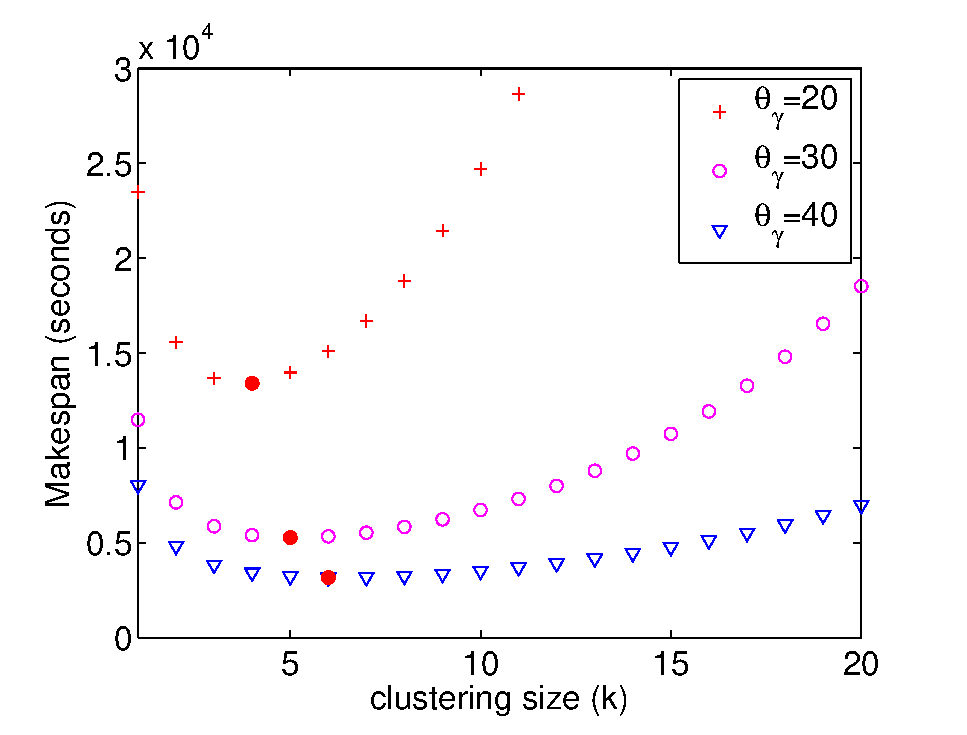
\includegraphics[width=0.75\linewidth]{model_makespan.eps}
  \caption{Makespan with different clustering size and $\theta_{\gamma}$. ($n=1000$, $r=20$, $\theta_t=5$ sec, $\theta_s=50$ sec). The red dots are the minimums. }
  \label{fig:model_makespan}
\end{figure*}

\begin{figure*}[!htb]
\centering
  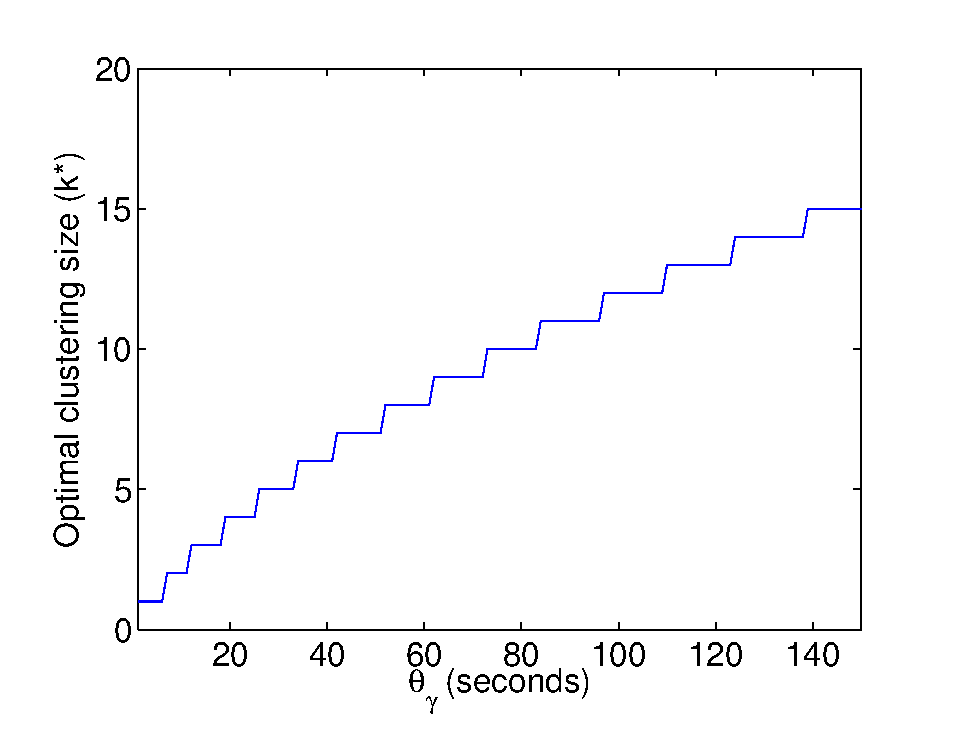
\includegraphics[width=0.75\linewidth]{model_size.eps}
  \caption{Optimal clustering size (k*) with different  $\theta_{\gamma}$ ($n=1000$, $r=20$, $\theta_t=5$ sec, $\theta_s=50$ sec)}
  \label{fig:model_size}
\end{figure*}


From this theoretic analysis, we conclude that (\emph{i}) the longer the inter-arrival time of failures is, the better runtime performance the task clustering has; (\emph{ii}), adjusting the clustering size according to the detected inter-arrival time can improve the runtime performance. 

\section{Fault Tolerant Clustering}
\label{sec:clustering}

As indicated in Section \ref{sec:model}, inappropriate clustering may increase the makespan of executing a workflow. To improve the fault tolerance from the point of view of clustering, we propose three methods: Dynamic Reclustering (\emph{DR}), Selective Reclustering (\emph{SR}) and Vertical Reclustering (\emph{VR}). In the experiments, we compare the performance of our fault tolerant clustering methods to an existing version of Horizontal Clustering (HC)~\cite{Singh2008} technique. In this subsection, we first briefly describe this algorithm.

\textbf{Horizontal Clustering} (\emph{HC}). 
Horizontal Clustering (HC) merges multiple tasks that are at the same horizontal level of the workflow. The clustering granularity (number of tasks within a cluster) of a clustered job is controlled by the user, who defines either the number of tasks per clustered job (\emph{clusters.size}), or the number of clustered jobs per horizontal level of the workflow (\emph{clusters.num}). This algorithm has been implemented and used in Pegasus~\cite{Singh2008}. For simplicity, we define \emph{clusters.num} as the number of available resources. In our prior work~\cite{Chen2013a,Chen2013b}, we have compared the runtime performance with different clustering granularity. The pseudocode of the HC technique is shown in Algorithm~\ref{alg:evaluation_hc}. The Clustering and Merge Procedure are called in the initial task clustering process while the Reclustering Procedure is called when there is a failed job returned. 

\begin{algorithm}[!htb]
	\footnotesize
	\caption{Horizontal Clustering algorithm.}
	\label{alg:evaluation_hc}
	\begin{algorithmic}[1]
		\Require $W$: workflow; $C$: max number of tasks per job defined by \emph{clusters.size} or \emph{clusters.num}
		\Procedure{Clustering}{$W,C$}
			\For{$level < depth(W)$}
				\State $TL\gets $\ \Call{GetTasksAtLevel}{$W,level$} \Comment{Partition $W$ based on depth}
				\State $CL\gets$  \ \Call{Merge}{$TL,C$} \Comment{Returns a list of clustered jobs}
				\State $W \gets W - TL + CL$  \Comment{Merge dependencies as well} 
			\EndFor
		\EndProcedure
		\Procedure{Merge}{$TL, C$}
			\State $J\gets$ \{\}\Comment{An empty job}
			\State $CL\gets$\{\}\Comment{An empty list of clustered jobs}
			\While{$TL$ is not empty}
				\State $J$.add ($TL$.pop($C$) \Comment{Pops $C$ tasks that are not merged }
				\State  $CL$.add( $J$)
			\EndWhile
			\State \textbf{return} $CL$
		\EndProcedure
		\Procedure{Reclustering}{$J$}\Comment{$J$ is a failed job}
			\State $J_{new}\gets$\ \Call{CopyOf}{$J$} \Comment{Copy Job $J$}
			\State $W \gets W + J_{new}$ \Comment{Reexecute it}
		\EndProcedure
	\end{algorithmic}
\end{algorithm}


\begin{figure*}[!htb]
\centering
  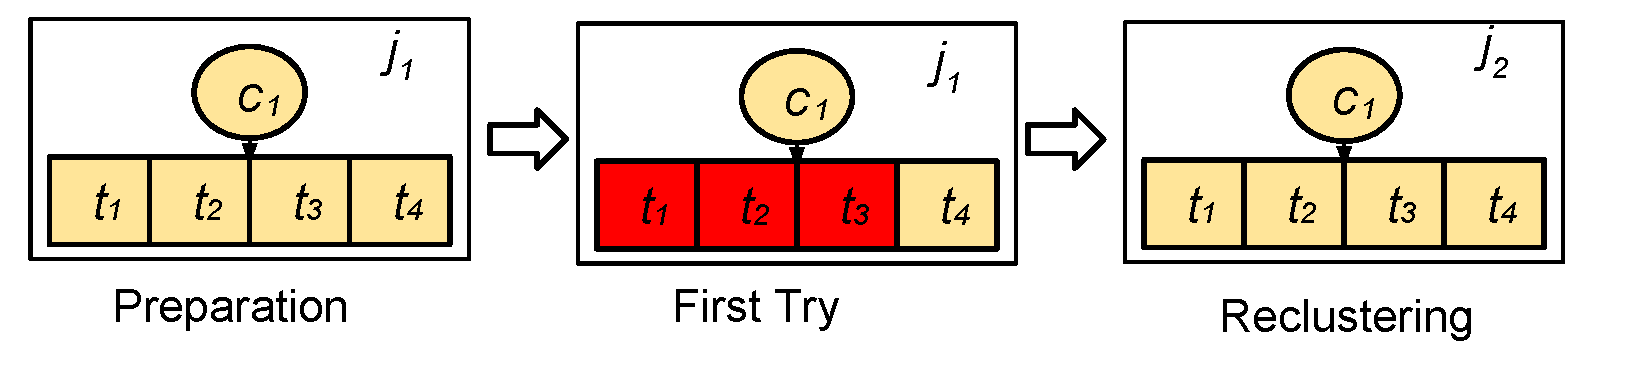
\includegraphics[width=0.55\linewidth]{hcr.pdf}
  \caption{Horizontal Clustering (red boxes are failed tasks)}
  \label{fig:clustering_hc}
\end{figure*}

%The type of tasks is used to detect the task specific failures and the resource id is used to detect location specific failures. 
Figure \ref{fig:clustering_hc} shows an example where the initial clustering size is 4 and thereby there are four tasks in a clustered job at the beginning. During execution, three out of these tasks ($t_1, t_2, t_3$) fail. HC will keep retrying all of the four tasks in next try until all of them succeed. Such a retry mechanism has been implemented and used in Pegasus~\cite{Singh2008}.




\begin{figure*}[!htb]
\centering
  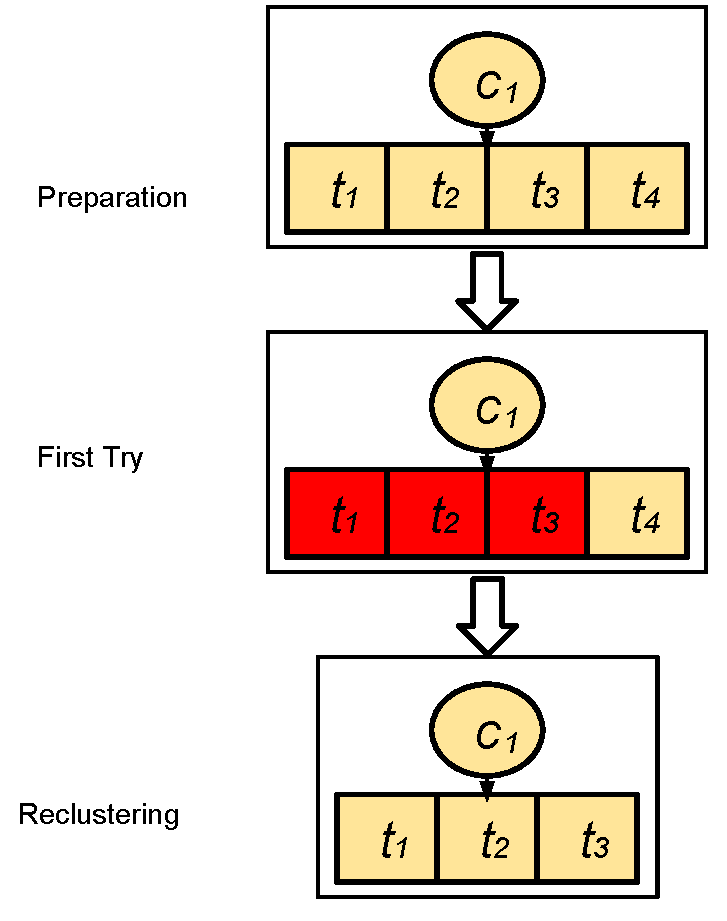
\includegraphics[width=0.55\linewidth]{sr.pdf}
  \caption{Selective Reclustering (red boxes are failed tasks)}
  \label{fig:clustering_sr}
\end{figure*}

\textbf{Selective Reclustering} (\emph{SR}). In HC, the clustering engine does not adjust the clustering size even when it continuously sees many failures. We further improve the performance with Selective Reclustering that selects the failed tasks in a clustered job and merges them into a new clustered job. SR is different to the HC in that the latter method retries all tasks of a failed job even though some of the tasks have succeeded. SR requires task level monitoring in workflow management systems. 

Figure \ref{fig:clustering_sr} shows an example of SR. At the first try, there are four tasks and three of them ($t_1, t_2, t_3$) have failed. One task ($t_4$) succeeds and exits. Only the three failed tasks are merged again into a new clustered job $j_2$ and the job is retried. This approach does not intend to adjust the clustering size, although the clustering size will be smaller and smaller spontaneously after each retry since there are less and less tasks in a clustered job. In this case, the clustering size has decreased from 4 to 3. However, the optimal clustering size may not be 3, which limits its performance if the $\theta_{\gamma}$ is small and $k$ should be decreased as much as possible. The advantage of SR is that it is simple to implement and be incorporated into existing workflow management systems without loss of much efficiency as shown in Section~\ref{sec:experiments}. It also serves as a comparison with the Dynamic Reclustering approach that we propose below. Algorithm \ref{alg:evaluation_sr} shows the pseudocode of SR. The Clustering and Merge procedures are the same as those in HC. 

\begin{algorithm}[!htb]
	\footnotesize
	\caption{Selective Reclustering algorithm. }
	\label{alg:evaluation_sr}
	\begin{algorithmic}[1]
		\Require $W$: workflow; $C$: max number of tasks per job defined by \emph{clusters.size} or \emph{clusters.num}
			\Procedure{Reclustering}{$J$}\Comment{$J$ is a failed job}
			\State $TL \gets$\ \Call{GetTasks}{$J$}
			\State $J_{new}\gets$\{\}\Comment{An empty job}
			\ForAll{Task $t$ in $TL$}
				\If{$t$ is failed}
					\State $J_{new}$.add ($t$)
				\EndIf
			\EndFor
			\State $W \gets W + J_{new}$ \Comment{Reexecute it}
		\EndProcedure
	\end{algorithmic}
\end{algorithm}

 

\begin{figure*}[!htb]
\centering
  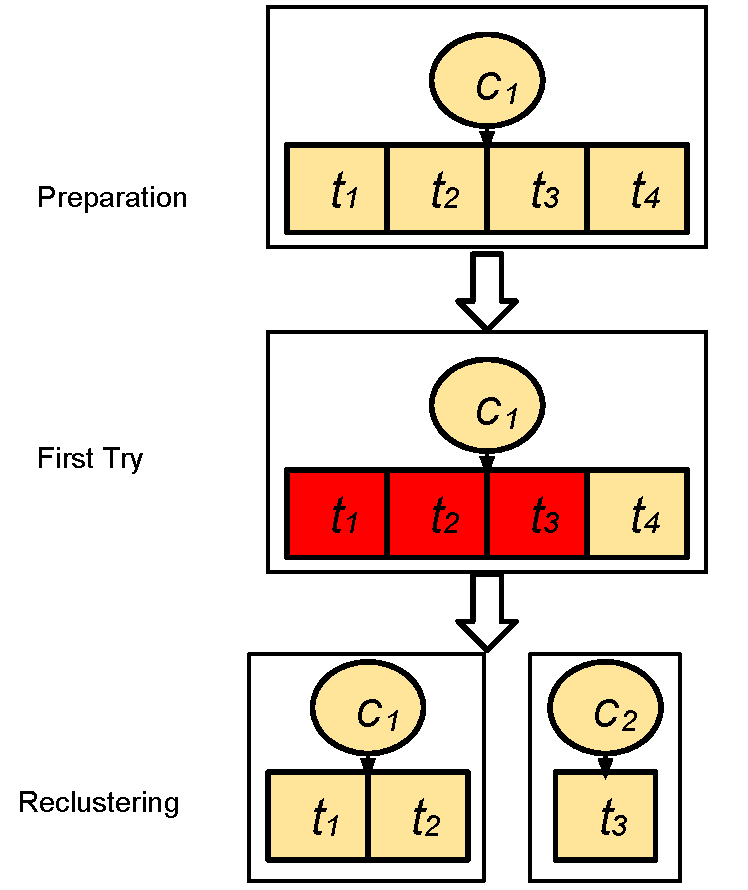
\includegraphics[width=0.55\linewidth]{dr.pdf}
  \caption{Dynamic Reclustering (red boxes are failed tasks)}
  \label{fig:clustering_dr}
\end{figure*}

\textbf{Dynamic Reclustering} (\emph{DR}). 
Selective Reclustering does not analyze the clustering size rather, it uses a self-adjusted approach to reduce the clustering size if the failure rate is too high. However, it is blind about the optimal clustering size and the actual clustering size may be larger or smaller than the optimal clustering size. We then propose the second method, Dynamic Reclustering. In DR, only failed tasks are merged into new clustered jobs and the clustering size is set to be $k^*$ according to Equation \ref{eq:k_optimal}. DR requires the ability to detect which tasks have failed in a job. 



Figure \ref{fig:clustering_dr} shows an example where the initial clustering size is 4 and thereby there are four tasks in a clustered job at the beginning. At the first try, three tasks within a clustered job have failed. Therefore we have only three tasks to retry and further we need to decrease the clustering size (in this case it is 2) accordingly. We end up with two new jobs $j_2$ (that has $t_1$ and $t_2$) and $j_3$ that has $t_3$. Algorithm \ref{alg:evaluation_dr} shows the pseudocode of DR. The Clustering and Merge procedures are the same as those in HC. 

\begin{algorithm}[!htb]
	\footnotesize
	\caption{Dynamic Reclustering algorithm.}
	\label{alg:evaluation_dr}
	\begin{algorithmic}[1]
		\Require $W$: workflow; $C$: max number of tasks per job defined by \emph{clusters.size} or \emph{clusters.num}
			\Procedure{Reclustering}{$J$}\Comment{$J$ is a failed job}
			\State $TL \gets$\ \Call{GetTasks}{$J$}
			\State $J_{new}\gets$\{\}
			\ForAll{Task $t$ in $TL$}
				\If{$t$ is failed}
					\State $J_{new}$.add ($t$)
				\EndIf
				\If{$J_{new}.size() > k^*$}
					\State $W \gets W + J_{new}$
					\State $J_{new}\gets$\{\}
				\EndIf
			\EndFor
			\State $W \gets W + J_{new}$ \Comment{Reexecute it}
		\EndProcedure
	\end{algorithmic}
\end{algorithm}

\begin{figure*}[!htb]
\centering
  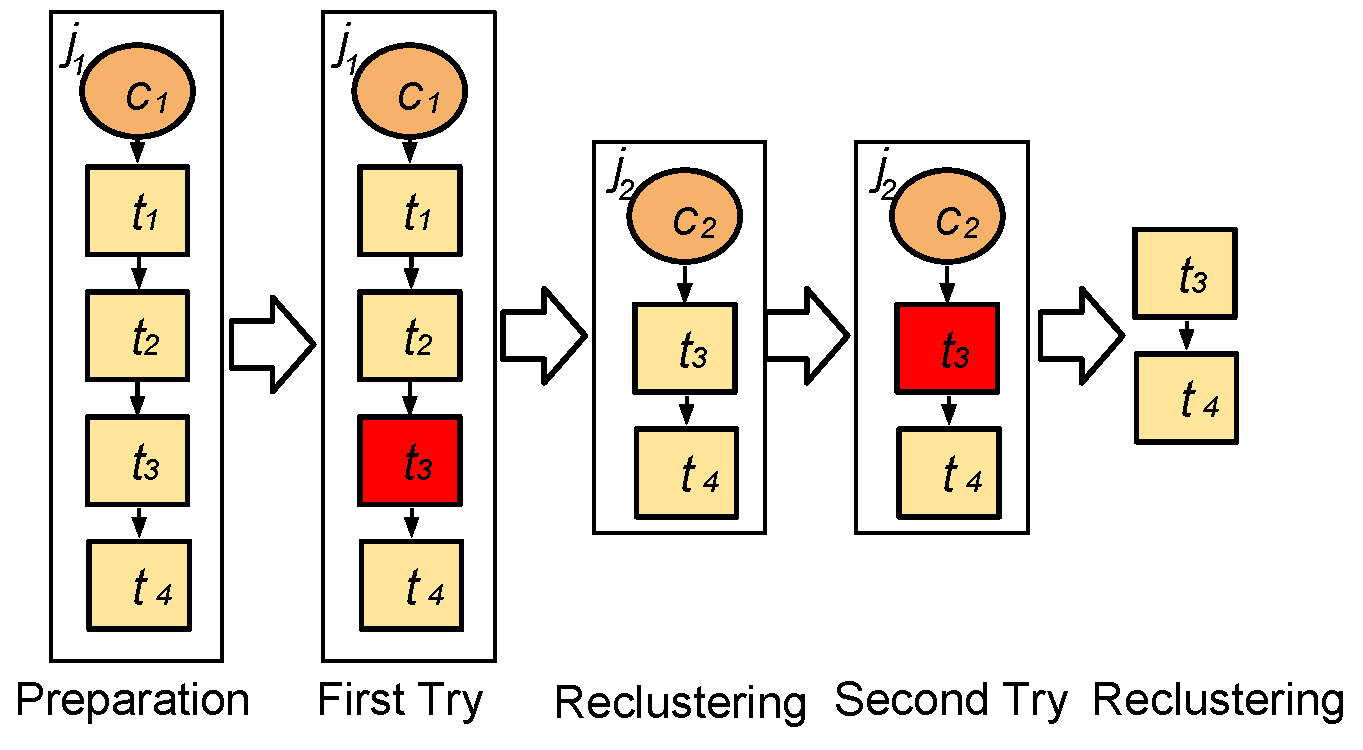
\includegraphics[width=0.85\linewidth]{vr.pdf}
  \caption{Vertical Reclustering (red boxes are failed tasks)}
  \label{fig:clustering_vr}
\end{figure*}

\textbf{Vertical Reclustering} (\emph{VR}). VR is an extension of Vertical Clustering. Similar to Selective Reclustering, Vertical Reclustering only retries failed tasks.
If there is a failure detected, we decrease $k$ by half and recluster them. In Figure \ref{fig:clustering_vr}, if there is no assumption of failures initially, we put all the tasks ($t_1, t_2, t_3, t_4$) from the same  pipeline into a clustered job. $t_3$ fails at the first try assuming it is a failure-prone task (its $\theta_{\gamma}$ is short). VR retries only the failed tasks ($t_3$) and tasks that are not completed ($t_4$) and merges them again into a new job $j_2$. In the second try, $j_2$ unfortunately fails and we divide it into two tasks ($t_3$ and $t_4$). Since the clustering size is already 1, VR performs no vertical clustering anymore and would continue retrying $t_3$ and $t_4$ (but still following their data dependency) until they succeed. Algorithm \ref{alg:evaluation_vr} shows the pseudocode of VR. 

\begin{algorithm}[!htb]
	\footnotesize
	\caption{Vertical Reclustering algorithm.}
	\label{alg:evaluation_vr}
	\begin{algorithmic}[1]
		\Require $W$: workflow; 
		\Procedure{Clustering}{$W$}
			\For{$level < depth(W)$}
				\State $TL\gets $\ \Call{GetTasksAtLevel}{$W,level$} \Comment{Partition $W$ based on depth}
				\State $CL, TL_{merged}\gets$  \ \Call{Merge}{$TL$} \Comment{Returns a list of clustered jobs}
				\State $W \gets W - TL_{merged} + CL$  \Comment{Merge dependencies as well} 
			\EndFor
		\EndProcedure
		\Procedure{Merge}{$TL$}
			\State $TL_{merged}\gets TL$\Comment{All the tasks that have been merged}
			\State $CL\gets$\{\}\Comment{An empty list of clustered jobs}
			\ForAll{$t$ in $TL$}
				\State $J\gets$ \{$t$\}
				\While{$t$ has only one child $t_{child}$}
					\State $J$.add ($t_{child}$)
					\State $TL_{merged}\gets TL_{merged} + t_{child}$ 
					\State $t\gets t_{child}$
				\EndWhile
				\State  $CL$.add( $J$)
			\EndFor
			\State \textbf{return} $CL$, $TL_{merged}$
		\EndProcedure
		\Procedure{Reclustering}{$J$}\Comment{$J$ is a failed job}
			\State $TL \gets$\ \Call{GetTasks}{$J$}
			\State $k^*\gets J.size() / 2$ \Comment{Reduce the clustering size by half}
			\State $J_{new}\gets$\{\}
			\ForAll{Task $t$ in $TL$}
				\If{$t$ is failed or not completed}
					\State $J_{new}$.add ($t$)
				\EndIf
				\If{$J_{new}.size() > k^*$}
					\State $W \gets W + J_{new}$
					\State $J_{new}\gets$\{\}
				\EndIf
			\EndFor
			\State $W \gets W + J_{new}$ \Comment{Reexecute it}
		\EndProcedure
	\end{algorithmic}
\end{algorithm}



\section{Experiments and Discussions}
\label{sec:experiments}


In this section, we evaluate our methods with five workflows, whose runtime information is gathered from real execution traces. The simulation-based approach allows us to control system parameters such as the inter-arrival time of task failures in order to clearly demonstrate the reliability of the algorithms. Our methods can also be applied to real workflow management systems as long as they support task-level failure monitoring. 

\subsection{Scientific workflow applications}
\label{sec:applications}

Five real scientific workflow applications are used in the experiments: LIGO Inspiral analysis~\cite{LIGO}, Montage~\cite{Berriman2004}, CyberShake~\cite{Graves2010}, Epigenomics~\cite{Epigenome}, and SIPHT~\cite{SIPHT}. In this subsection, we describe each workflow application and present their main characteristics and structures.

\paragraph{\textbf{LIGO}}
\begin{figure*}[!htb]
	\centering
	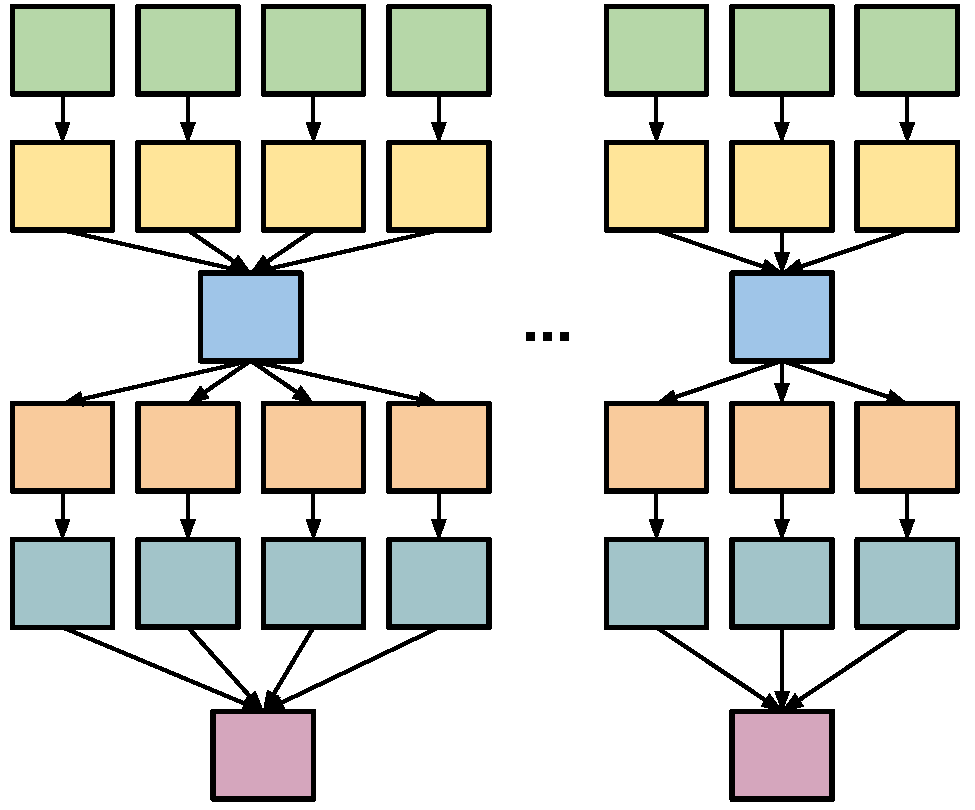
\includegraphics[width=0.5\linewidth]{ligo_shape.pdf} \\
	\caption{A simplified visualization of the LIGO Inspiral workflow.}
	\label{fig:evaluation_shape_ligo}
\end{figure*}
Laser Interferometer Gravitational Wave Observatory (LIGO)~\cite{LIGO} workflows are used to search for gravitational wave signatures in data collected by large-scale interferometers. The observatories' mission is to detect and measure gravitational waves predicted by general relativity (Einstein's theory of gravity), in which gravity is described as due to the curvature of the fabric of time and space. The LIGO Inspiral workflow is a data-intensive workflow. Figure~\ref{fig:evaluation_shape_ligo} shows a simplified version of this workflow. The LIGO Inspiral workflow is separated into multiple groups of interconnected tasks, which we call branches in the rest of our paper. However, each branch may have a different number of pipelines as shown in Figure~\ref{fig:evaluation_shape_ligo}. 

\begin{figure*}[htb]
	\centering
	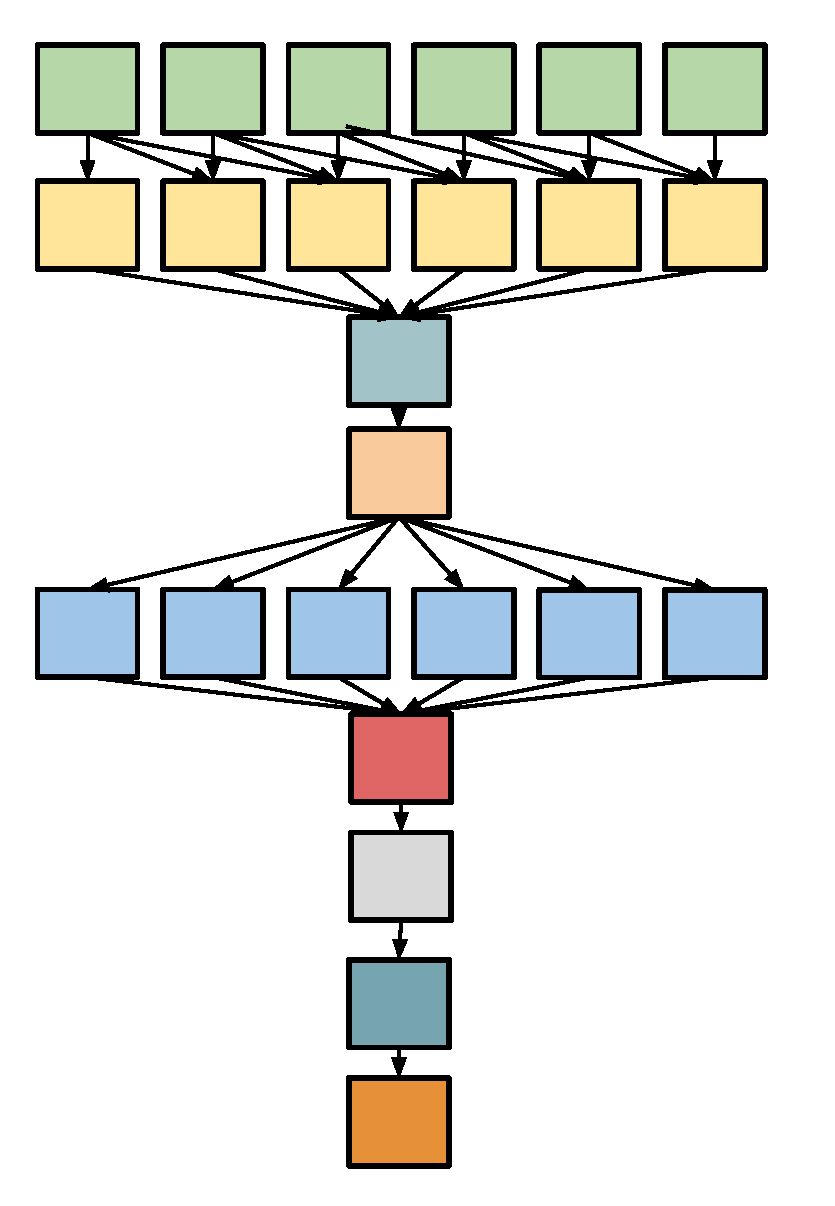
\includegraphics[width=0.45\linewidth]{montage_shape.pdf} \\
	\caption{A simplified visualization of the Montage workflow.}
	\label{fig:evaluation_shape_montage}
\end{figure*}

\paragraph{\textbf{Montage}}
Montage~\cite{Berriman2004} is an astronomy application that is used to construct large image mosaics of the sky. Input images are reprojected onto a sphere and overlap is calculated for each input image. The application re-projects input images to the correct orientation while keeping background emission level constant in all images. The images are added by rectifying them to a common flux scale and background level. Finally the reprojected images are co-added into a final mosaic. The resulting mosaic image can provide a much deeper and detailed understanding of the portion of the sky in question. Figure~\ref{fig:evaluation_shape_montage} illustrates a small Montage workflow. The size of the workflow depends on the number of images used in constructing the desired mosaic of the sky. 
%The structure of the workflow changes to accommodate increases in the number of inputs, which corresponds to an increase in the number of computational tasks.

\begin{figure*}[htb]
	\centering
	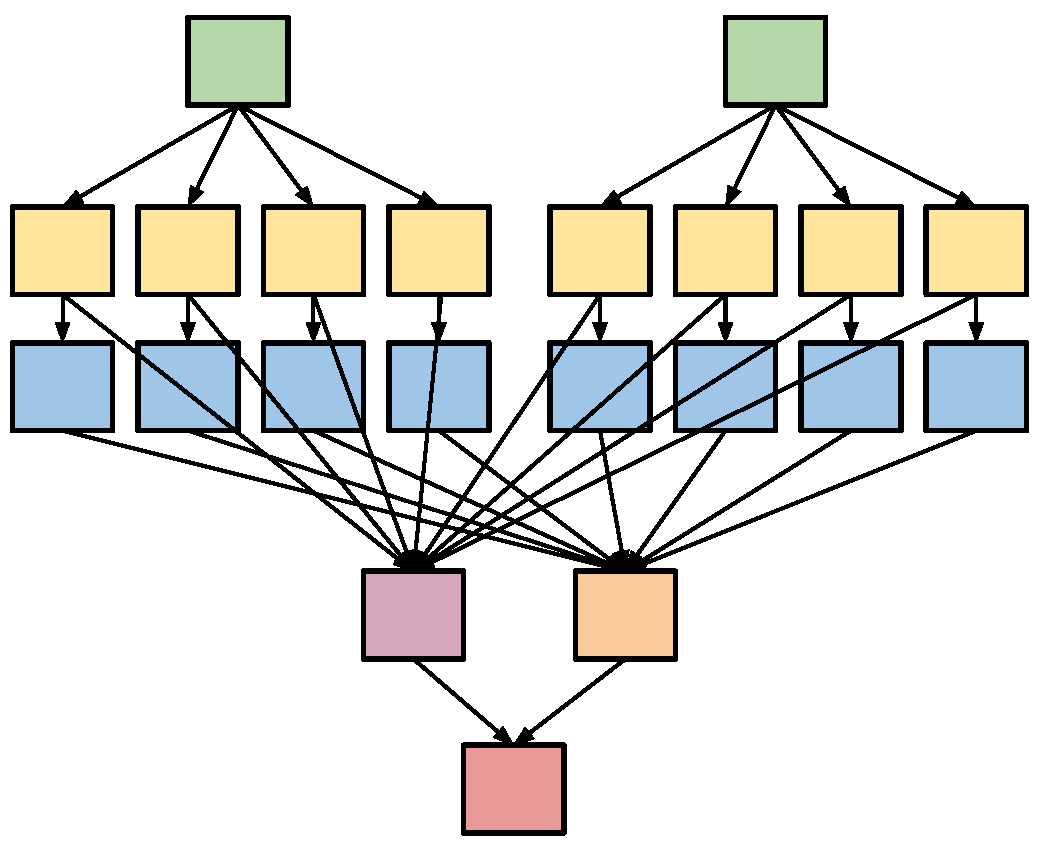
\includegraphics[width=0.55\linewidth]{cybershake_shape.pdf} \\
	\caption{A simplified visualization of the CyberShake workflow.}
	\label{fig:evaluation_shape_cybershake}
\end{figure*}

\paragraph{\textbf{Cybershake}}
CyberShake~\cite{Graves2010} is a seismology application that calculates Probabilistic Seismic Hazard curves for geographic sites in the Southern California region. It identifies all ruptures within 200km of the site of interest and converts rupture definition into multiple rupture variations with differing hypocenter locations and slip distributions. It then calculates synthetic seismograms for each rupture variance, and peak intensity measures are then extracted from these synthetics and combined with the original rupture probabilities to produce probabilistic seismic hazard curves for the site. Figure~\ref{fig:evaluation_shape_cybershake} shows an illustration of the Cybershake workflow.

\begin{figure*}[htb]
	\centering
	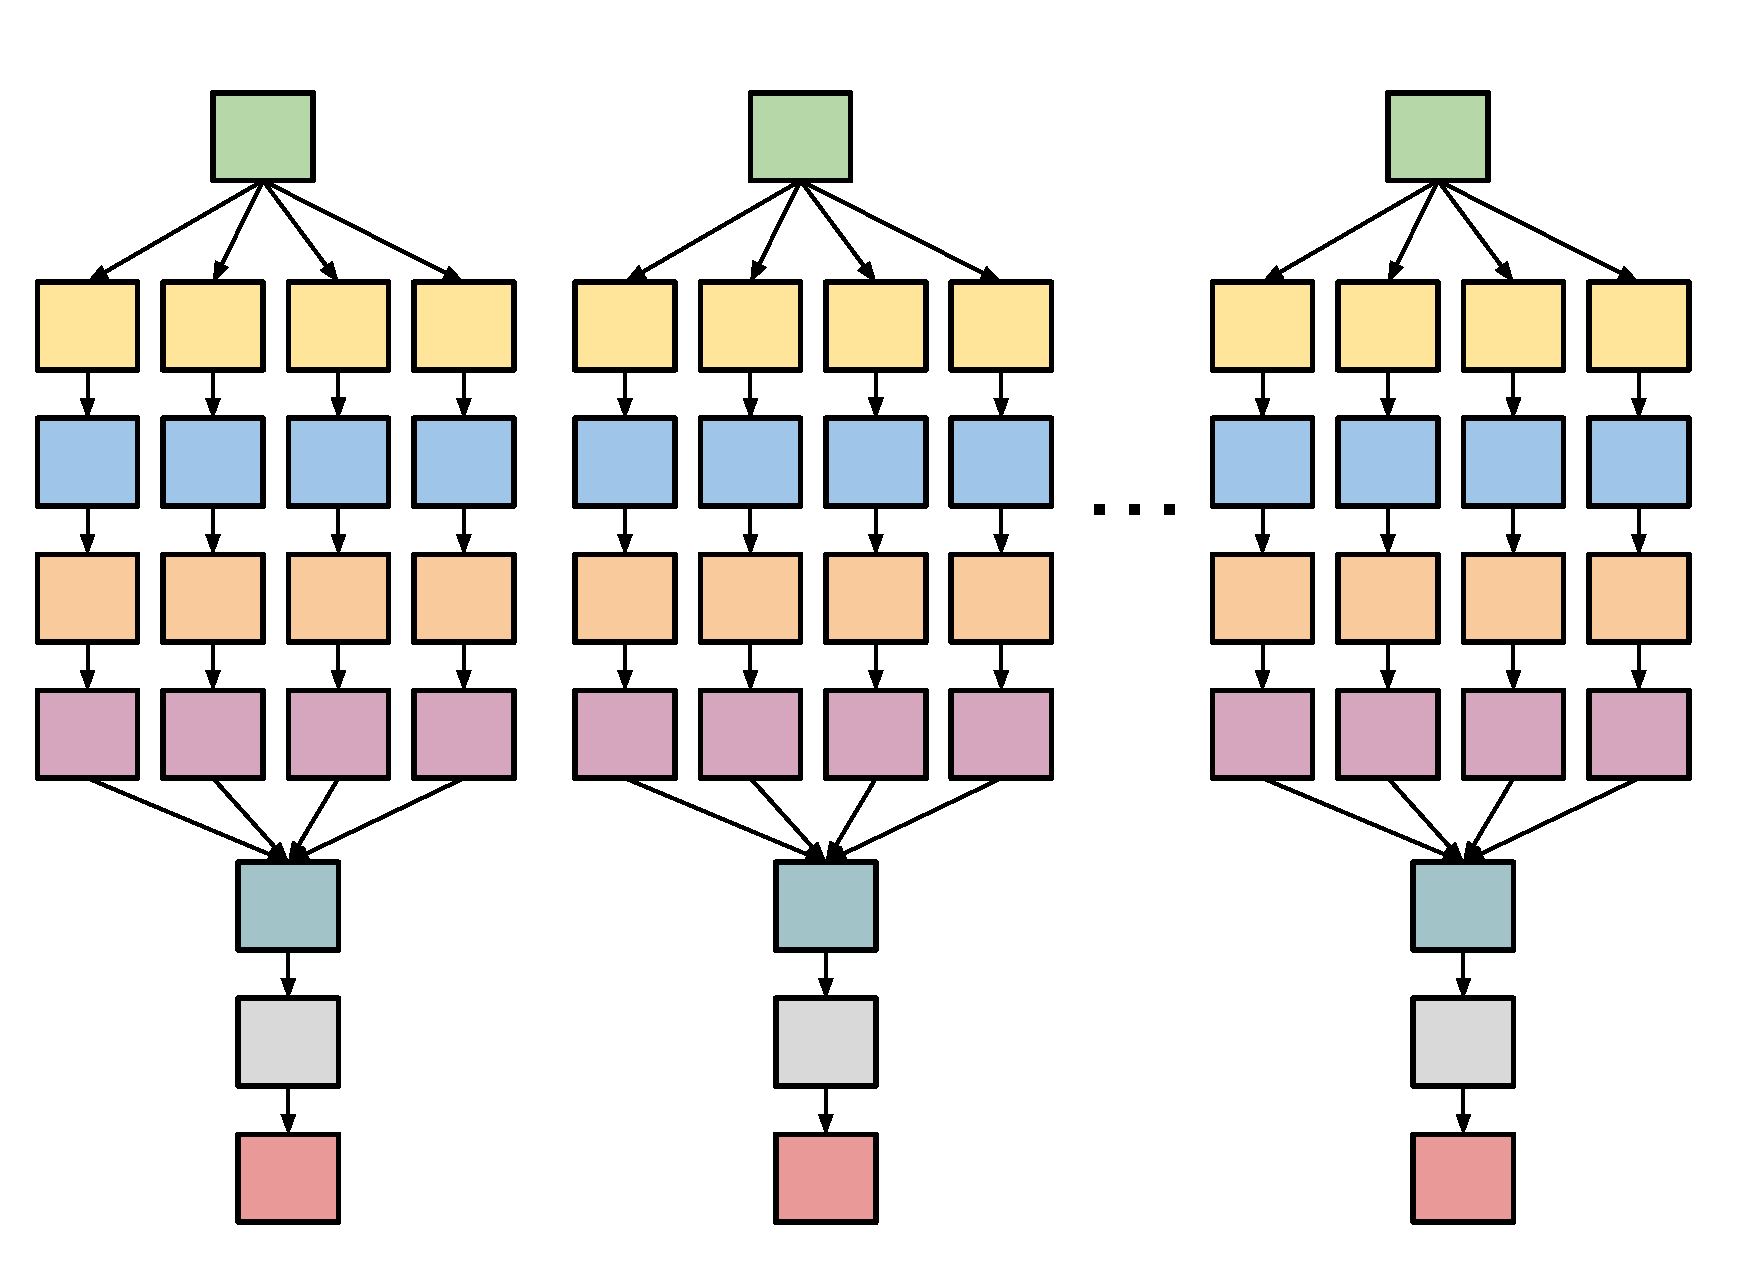
\includegraphics[width=0.8\linewidth]{genome_shape.pdf} \\
	\caption{A simplified visualization of the Epigenomics workflow with multiple branches.}
	\label{fig:evaluation_shape_genome}
\end{figure*}

\paragraph{\textbf{Epigenomics}}
The Epigenomics workflow~\cite{Epigenome} is a data-parallel workflow. Initial data are acquired from the Illumina-Solexa Genetic Analyzer in the form of DNA sequence lanes. Each Solexa machine can generate multiple lanes of DNA sequences. These data are converted into a format that can be used by sequence mapping software. The mapping software can do one of two major tasks. It either maps short DNA reads from the sequence data onto a reference genome, or it takes all the short reads, treats them as small pieces in a puzzle and then tries to assemble an entire genome. In our experiments, the workflow maps DNA sequences to the correct locations in a reference Genome. This generates a map that displays the sequence density showing how many times a certain sequence expresses itself on a particular location on the reference genome. Epigenomics is a CPU-intensive application and its simplified structure is shown in Figure~\ref{fig:evaluation_shape_genome}. 
%Different to the LIGO Inspiral workflow, each branch in Epigenomics has exactly the same number of pipelines, which makes it more symmetric. 

\begin{figure*}[htb]
	\centering
	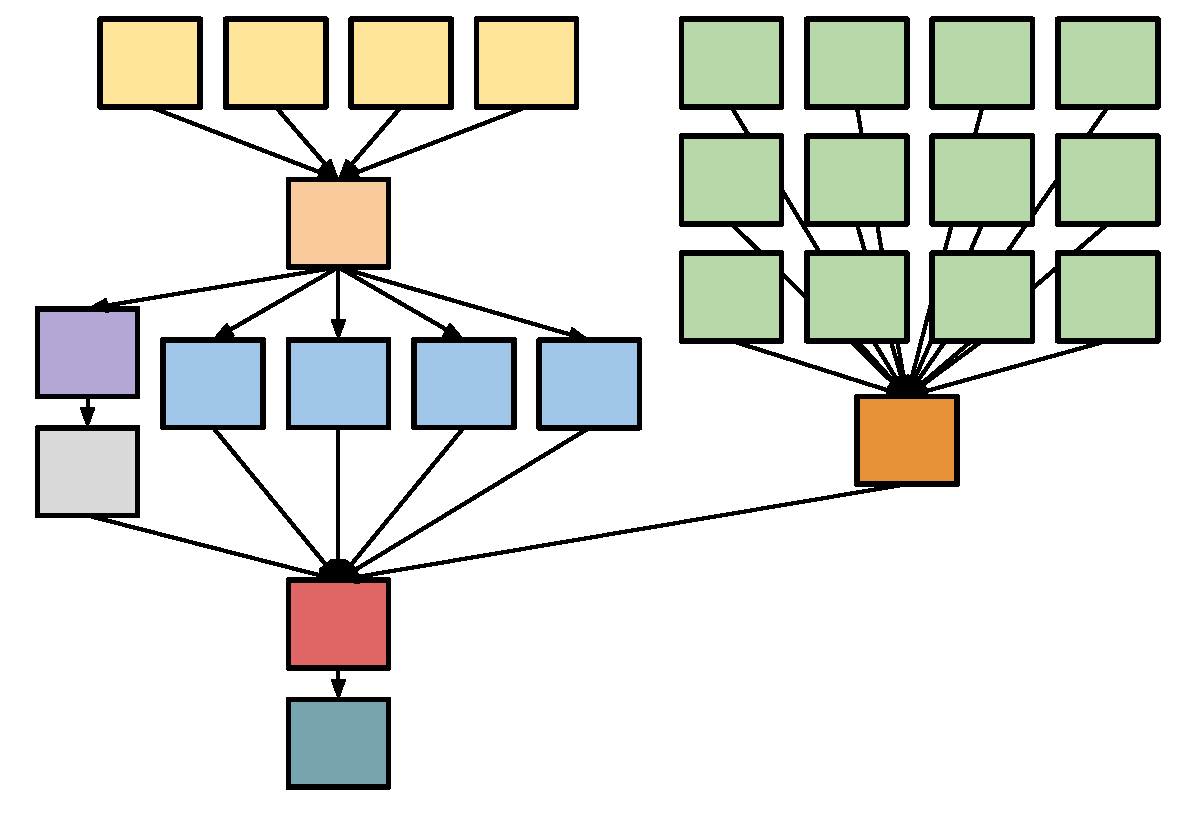
\includegraphics[width=0.6\linewidth]{sipht_shape.pdf} \\
	\caption{A simplified visualization of the SIPHT workflow.}
	\label{fig:evaluation_shape_sipht}
\end{figure*}

\paragraph{\textbf{SIPHT}}
The SIPHT workflow~\cite{SIPHT} conducts a wide search for small untranslated RNAs (sRNAs) that regulates several processes such as secretion or virulence in bacteria. The kingdom-wide prediction and annotation of sRNA encoding genes involves a variety of individual programs that are executed in the proper order using Pegasus~\cite{Deelman2004}. These involve the prediction of $\rho$-independent transcriptional terminators, BLAST (Basic Local Alignment Search Tools~\cite{BLAST}) comparisons of the inter genetic regions of different replicons and the annotations of any sRNAs that are found. A simplified structure of the SIPHT workflow is shown in Figure~\ref{fig:evaluation_shape_sipht}. 




\begin{table}[!htb]
	\setlength{\tabcolsep}{11pt}
	\centering
	\small
	\begin{tabular}{lrrrr}
		\hline
		 & \multicolumn{1}{c}{Number} & \multicolumn{1}{c}{Average} &  \multicolumn{1}{c}{Average} \\
		Workflow	& of Tasks	 & Data Size & Task Runtime \\
		\hline
		LIGO 		&800		& 5 MB	& 228s\\
		Montage 		&300		&3 MB	&11s\\
		CyberShake 	&700		&148 MB 	& 23s\\
		Epigenomics 	&165 	& 355 MB	& 2952s\\
		SIPHT		&1000	& 360 KB 	& 180s\\
		\hline
	\end{tabular}
	\caption{Summary of the scientific workflows characteristics.}
	\label{tab:evaluation_workflows}
\end{table} 

Table~\ref{tab:evaluation_workflows} shows the summary of the main \textbf{workflows characteristics}: number of tasks, average data size, and average task runtimes for the five workflows. 


% Experiment conditions
\subsection{Experiment conditions}
\label{sec:experiment_conditions}
We adopt a trace-based simulation approach, where we extended our WorkflowSim~\cite{WorkflowSim} simulator with the fault tolerant clustering methods to simulate a controlled distributed environment. WorkflowSim is an open source workflow simulator that extends CloudSim~\cite{Calheiros2011} by providing support for task clustering, task scheduling, and resource provisioning at the workflow level. It has been recently used in multiple workflow study areas~\cite{WorkflowSim,Chen2012, jrad2013broker} and its correctness has been verified in~\cite{WorkflowSim}. 

The simulated computing platform is composed by 20 single homogeneous core virtual machines (worker nodes), which is the quota per user of some typical distributed environments such as Amazon EC2~\cite{AmazonAWS} and FutureGrid~\cite{FutureGrid}. Amazon EC2 is a commercial, public cloud that has been widely used in distributed computing, in particular for scientific workflows~\cite{Berriman2010}. FutureGrid is a distributed, high-performance testbed that provides scientists with a set of computing resources to develop parallel, grid, and cloud applications. Each simulated virtual machine (VM) has 512MB of memory and the capacity to process 1,000 million instructions per second. The default network bandwidth is 15MB according to the real environment in FutureGrid from where our traces were collected. By default, we merge tasks at the same horizontal level into 20 clustered jobs initially, which is a simple selection of granularity control of the strength of task clustering. The study of granularity size has been done in~\cite{Chen2013b}, which shows such selection is acceptable. 

We collected workflow execution traces~\cite{Juve2013, Chen2011} (including overhead and task runtime information) from real runs (executed on FutureGrid and Amazon EC2) of the scientific workflow applications described in Section~\ref{sec:applications}. The traces are used to feed the Workflow Generator toolkit~\cite{WorkflowGenerator} to generate synthetic workflows. This allows us to perform simulations with several different configurations under controlled conditions. The toolkit uses the information gathered from actual scientific workflow executions to generate synthetic workflows resembling those used by real world scientific applications. The number of inputs to be processed, the number of tasks in the workflow, and their composition determine the structure of the generated workflow. Such an approach of traced based simulation allows us to utilize real traces and vary the system setting (i.e., the inter-arrival time of failures) and workflow (i.e., avg. task runtime) to fully explore the performance of our fault tolerant clustering algorithms. 

Three sets of experiments are conducted. Experiment 1 evaluates the performance of our fault tolerant clustering methods (DR, VR, and SR) over a baseline execution (HC) that is not fault tolerant for the five workflows. The goal of the experiment is to identify conditions where each method works best and worst. In addition, we also evaluate the performance improvement under different $\theta_{\gamma}$ (the inter-arrival time of task failures). The range of $\theta_{\gamma}$ is chosen from 10x to 1x of the average task runtime such that the workflows do not run forever and we can visualize the performance difference better. 


Experiment 2 evaluates the performance impact of the variation of the average task runtime per level (defined as the average of all the tasks per level) and the average system overheads per level for one scientific workflow application (CyberShake). In particular, we are interested in the performance of DR based on the results of Experiment 1 and we use $\theta_{\gamma}=100$ since it has the maximum difference between the four methods. The original average task runtime of all the tasks of the CyberShake workflow is about 23 seconds as shown in Table~\ref{tab:evaluation_workflows}. In this experiment, we multiply the average task runtime by a multiplier from 0.5 to 1.3. The scale parameter of the system overheads ($\theta_{s}$) is 50 seconds originally based on our traces and we multiply the system overheads by a multiplier from 0.2 to 1.8.  

Experiment 3 evaluates the performance of dynamic estimation and static estimation. In the static estimation process, we only use the prior knowledge to estimate the MLEs of $\theta_t$, $\theta_s$ and $\theta_{\gamma}$. In the dynamic estimation process, we also leverage the runtime data collected during the execution and update the MLEs respectively. In this experiment, we decrease $\theta_{\gamma}$ from 500 seconds to 50 seconds at time $T$ to simulate the scenario where there are more failures coming than expected. Theoretically speaking, the later we change $\theta_{\gamma}$, the less the reclustering is influenced by the estimation error and thus the less the makespan is. There is one special case when $T\to 0$, which means the prior knowledge is wrong at the very beginning. 

Table~\ref{tab:evaluation_methods} summarizes the clustering methods to be evaluated in our experiments. . 
\begin{table}[!htb]
	%\setlength{\tabcolsep}{11pt}
	\centering
	\small
	\begin{tabular}{l|rrrr}
		\hline
		Abbreviation	& Method	  \\
		\hline
		DR 		& Dynamic Reclustering		\\
		SR 		&Selective Reclustering\\
		VR 	&Vertical Reclustering\\
		HC 	&Horizontal Clustering \\
		\hline
	\end{tabular}
	\caption{Methods to Evaluate in Experiements}
	\label{tab:evaluation_methods}
\end{table} 


\subsection{Results and discussion}
\label{sec:results}

\begin{figure}[!htb]
\centering
  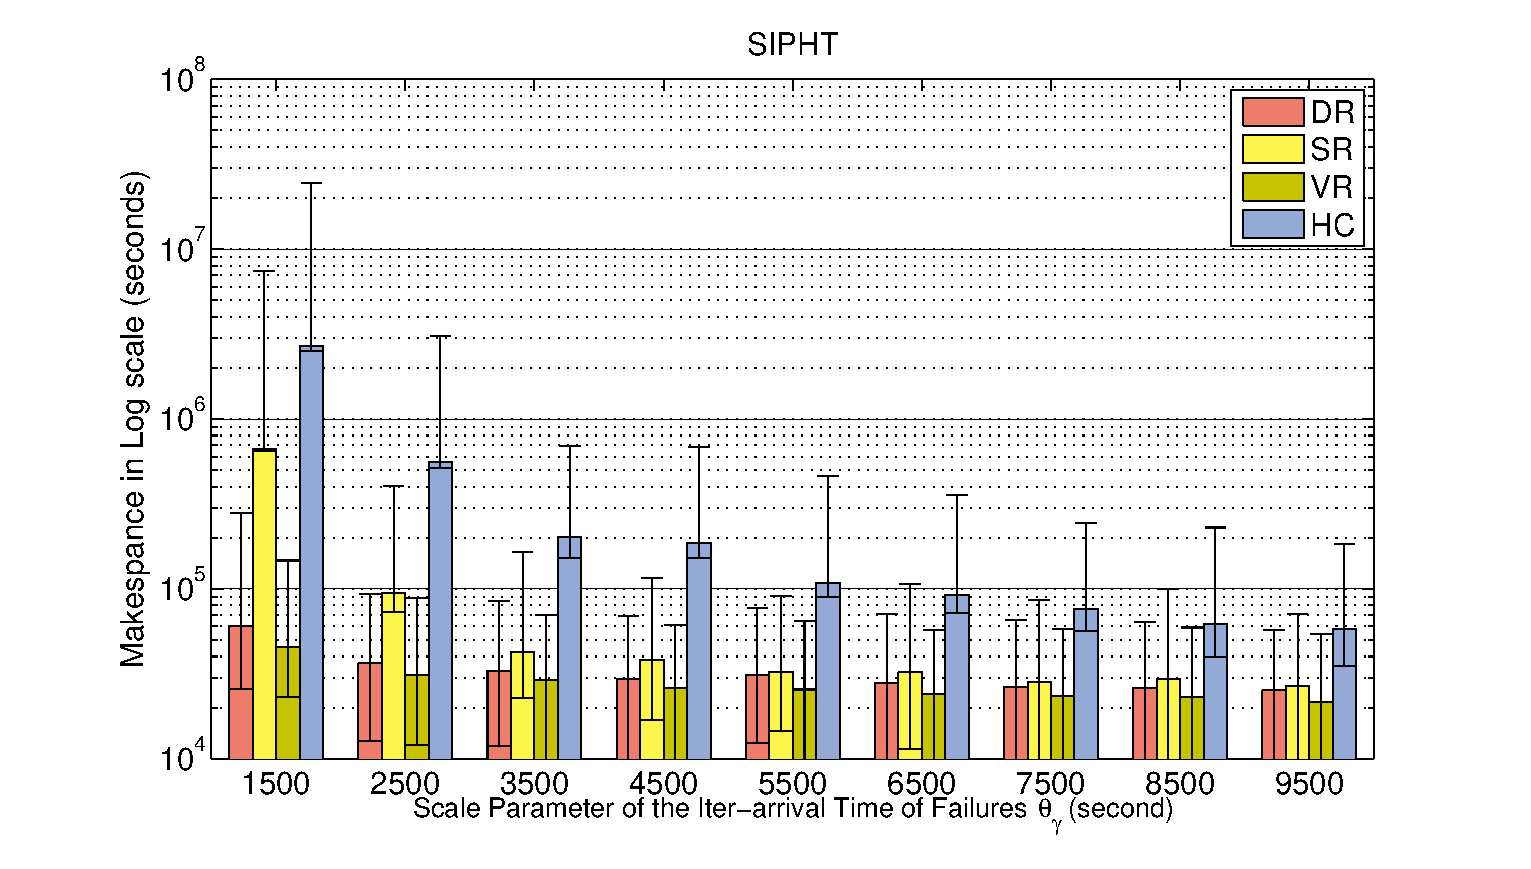
\includegraphics[width=1\linewidth]{sipht.eps}
  \caption{Experiment 1: SIPHT Workflow}
  \label{fig:expr_sipht}
\end{figure}

\paragraph{\textbf{Experiment 1}}
Figure~\ref{fig:expr_sipht}, \ref{fig:expr_genome}, \ref{fig:expr_cybershake}, \ref{fig:expr_ligo} and \ref{fig:expr_montage} show the performance of the four reclustering methods (DR, SR, VR and HC) with five workflows respectively. We draw conclusions: 

\begin{figure}[!htb]
\centering
  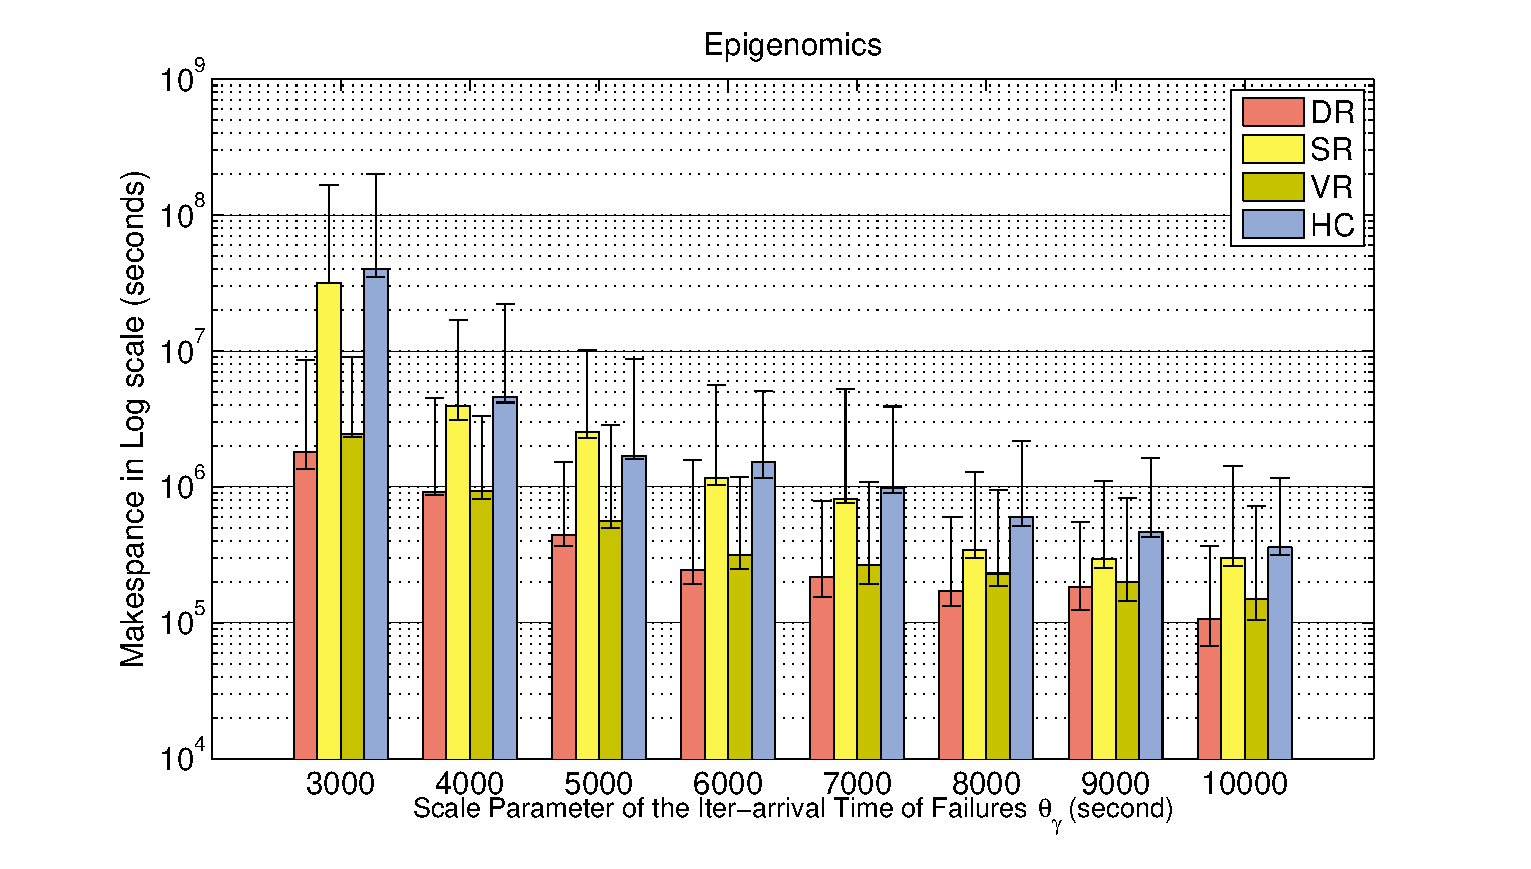
\includegraphics[width=1.0\linewidth]{genome.eps}
  \caption{Experiment 1: Epigenomics Workflow}
  \label{fig:expr_genome}
\end{figure}


1). DR, SR and VR have significantly improved the makespan compared to HC in a large scale. By decreasing of the inter-arrival time ($\theta_{\gamma}$) and consequently more failures are generated, the performance difference becomes more significant. 


\begin{figure}[!htb]
\centering
  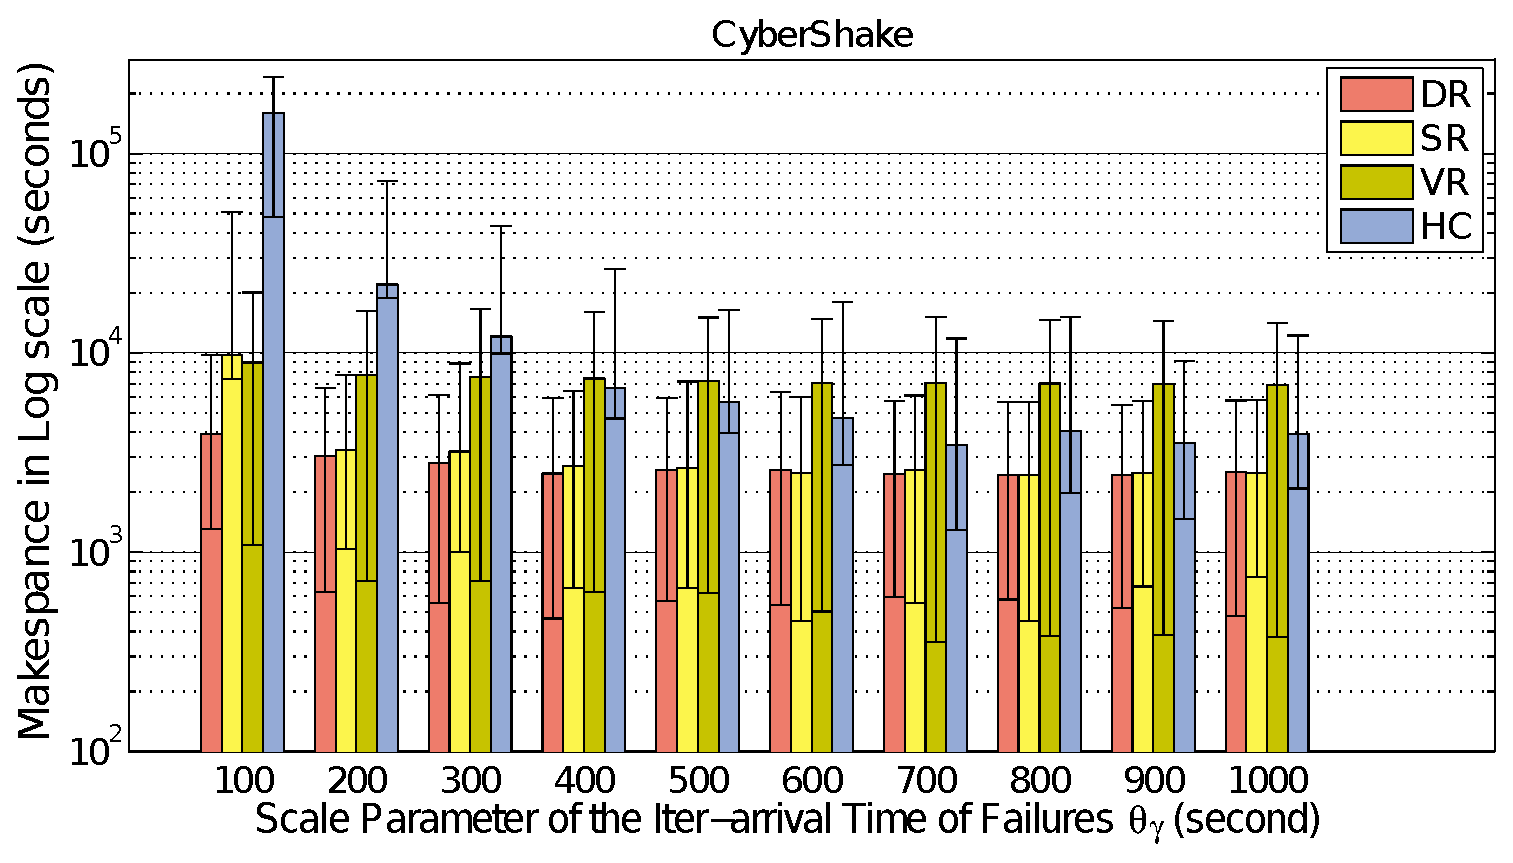
\includegraphics[width=1.0\linewidth]{cybershake.eps}
  \caption{Experiment 1: CyberShake Workflow}
  \label{fig:expr_cybershake}
\end{figure}






2). Among the three methods, DR and VR perform consistently better than SR, which fail to improve the makespan when $\theta_{\gamma}$ is small. The reason is the SR does not adjust $k$ according to the occurrence of failures. 
%It is more significant when there is a high failure rate ($\theta_{\gamma}$ is small). 

\begin{figure}[!htb]
\centering
  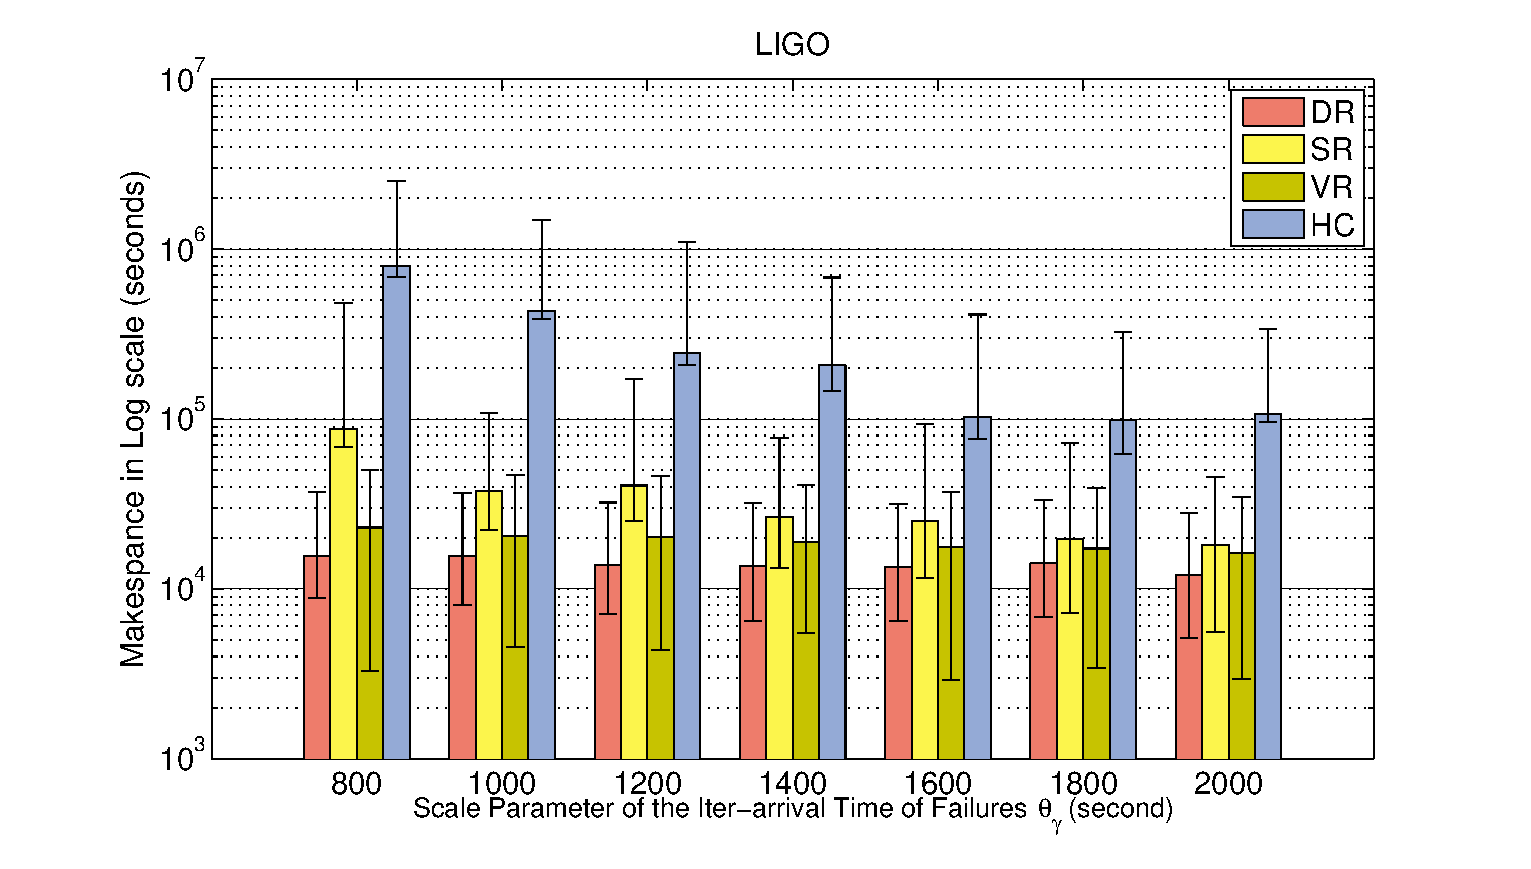
\includegraphics[width=1\linewidth]{ligo.eps}
  \caption{Experiment 1: LIGO Workflow}
  \label{fig:expr_ligo}
\end{figure}

3). The performance of VR is highly related to the workflow structure and the average task runtime. For example, according to Figure \ref{fig:evaluation_shape_genome} and Table \ref{tab:evaluation_workflows}, we know that the Epigenomics workflow has a long task runtime (around 50 minutes) and the pipeline length is 4. It means vertical clustering creates really long jobs ($50\times 4=200$ minutes, theoretically speaking) and thereby VR is more sensitive to the decrease of $\gamma$. As indicated in Figure \ref{fig:expr_genome}, the makespan increases more significantly with the decrease of $\theta_{\gamma}$ than other workflows. In comparison, the CyberShake workflow does not leave much space for vertical clustering methods to improve since it does not have many pipelines as shown in Figure~\ref{fig:evaluation_shape_cybershake}. In addition, the average task runtime of the CyberShake workflow is relatively short (around 23 seconds). Compared to horizontal methods such as HC, SR and DR, vertical clustering does not generate long jobs and thus the performance of VR is much less  sensitive to $\theta_{\gamma}$. 

%4). Under some cases, i.e., the CyberShake workflow, we see that VR does not perform well compared to DR or SR. The reason is the graph structure of the CyberShake workflow does not leave much space for vertical clustering methods to improve since it does not have many pipelines as shown in Figure~\ref{fig:evaluation_shape_cybershake}. DR, a modification of HC, is more likely to improve the performance since most of these workflows have many parallel tasks in the same level. 



\begin{figure}[!htb]
\centering
  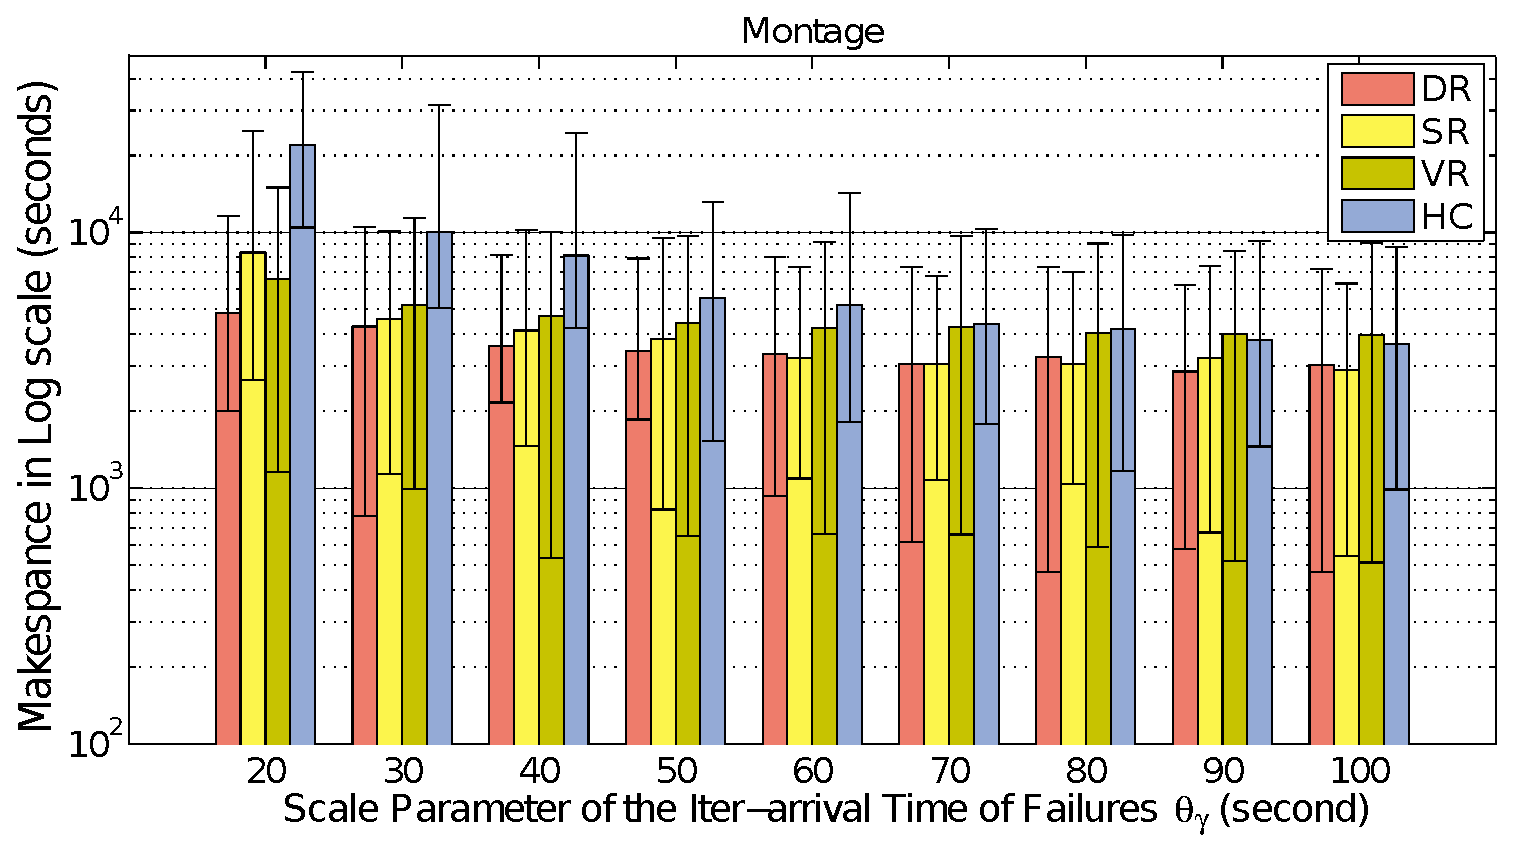
\includegraphics[width=1\linewidth]{montage.eps}
  \caption{Experiment 1: Montage Workflow}
  \label{fig:expr_montage}
\end{figure}

\paragraph{\textbf{Experiment 2}}

\begin{figure}[!htb]
\centering
  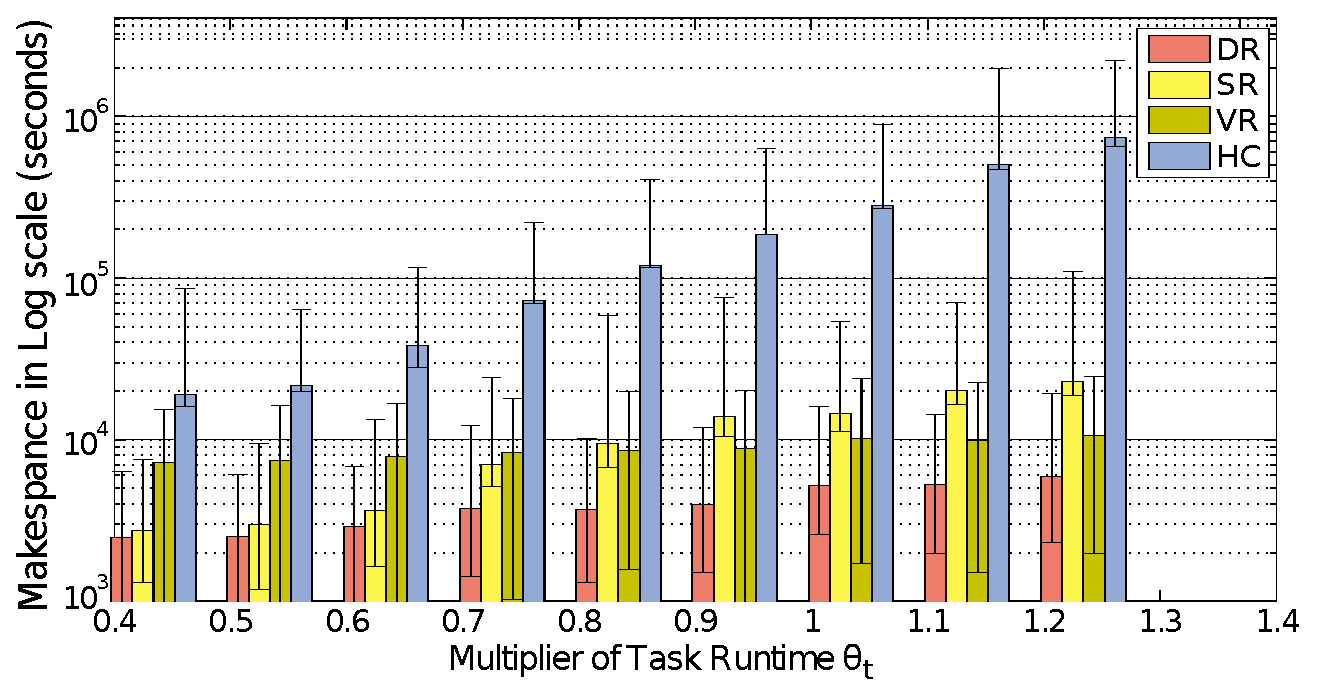
\includegraphics[width=1\linewidth]{t.eps}
  \caption{Experiment 2:  Influence of Varying Task Runtime on Makespan (CyberShake)}
  \label{fig:expr_t}
\end{figure}

Figure~\ref{fig:expr_t} shows the performance of our methods with different multiplier of $\theta_{t}$ for the CyberShake workflow. We can see that with the increase of the multiplier, the makespan increases significantly (increase from a scale of $10^4$ to $\sim 10^6$), particularly for HC. The reason is HC is not fault tolerant and it is sensitive to the increase of task runtime. While for DR, the reclustering process dynamically adjusts the clustering size based on the estimation of task runtime and thus the performance of DR is more stable. 
%VR?

\begin{figure}[!htb]
\centering
  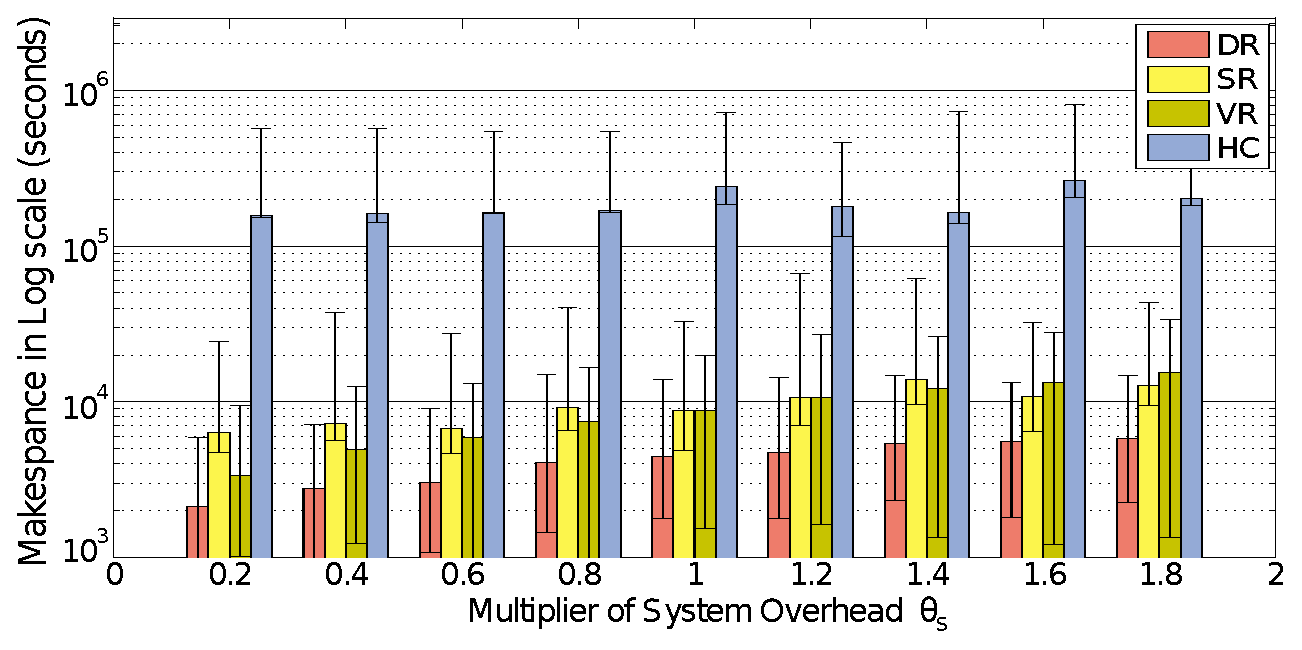
\includegraphics[width=1\linewidth]{d.eps}
  \caption{Experiment 2: Influence of Varying System Overhead on Makespan (CyberShake)}
  \label{fig:expr_d}
\end{figure}

Figure~\ref{fig:expr_d} shows the results with different multiplier of $\theta_{s}$ for the CyberShake workflow. Similarly, we can see that with the increase of the multiplier, the makespan increases for all the methods and DR performs best. However, the increase is less significant than that in Figure~\ref{fig:expr_t}. The reason is we may have multiple tasks in a clustered job but only one system overhead per job.


\paragraph{\textbf{Experiment 3}}
\begin{figure}[!htb]
\centering
  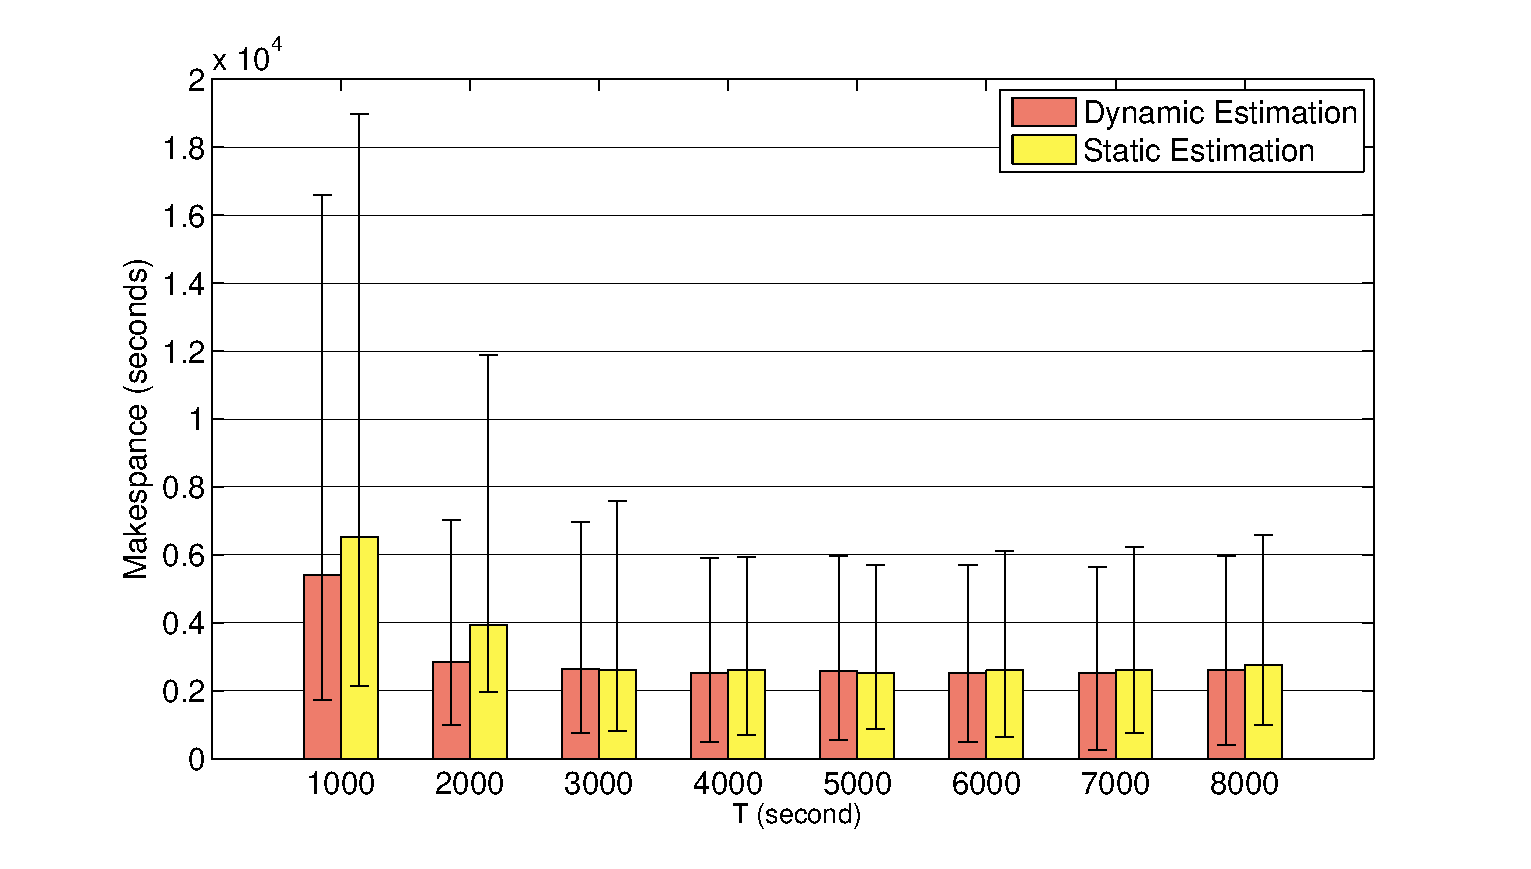
\includegraphics[width=1\linewidth]{versus.eps}
  \caption{Experiment 3: Static Estimation vs. Dynamic Estimation (CyberShake)}
  \label{fig:expr_static_dynamic}
\end{figure}

Figure~\ref{fig:expr_static_dynamic} further evaluates the performance of the dynamic estimation and static estimation for the CyberShake workflow. The reclustering method used in this experiment is DR since it performs best in the last two experiments. In the experiment, we change the inter-arrival time of failures ($\theta_{\gamma}$) from 500 seconds to 50 seconds at $T$. We can see that: 1). with the increase of $T$, both makespan decrease since the change of  $\theta_{\gamma}$ has less influence on the makespan and there is a lower failure rate on average; 2). Dynamic estimation improves the makespan by up to 34\% compared to the static estimation. The reason is the dynamic estimation is able to update the MLEs of the $\theta_{\gamma}$ and decrease the clustering size while the static estimation is not. 

\section{Conclusion and Future Work}

In this paper, we model transient failures in a distributed environment and propose three dynamic clustering methods to improve the fault tolerance of task clustering. We apply our methods to five widely used scientific workflows. From our experiments, we conclude that the three proposed methods improve the makespan significantly compared to an existing algorithm widely used in workflow management systems. In particular, our Dynamic Reclustering method performs best among the three methods since it can adjust the clustering size based on the Maximum Likelihood Estimation of task runtime, system overheads and the inter-arrival time of failures. Our Vertical Reclustering method improves the performance significantly for  workflows that have a short task runtime. Our dynamic estimation using on-going data collected from the workflow execution can further improve the fault tolerance in a dynamic environment where the inter-arrival time of failures is fluctuant. 

In this paper, we only discuss the fault tolerant clustering and apply it to a homogeneous environment. In the future, we aim to combine our work with fault tolerant scheduling in heterogeneous environments, i.e, a scheduling algorithm that avoids mapping clustered jobs to failure-prone nodes. We are also interested to combine vertical clustering methods with horizontal clustering methods. For example, we can perform vertical clustering either before or after horizontal clustering, which we believe would bring different performance improvement. 

\section{ACKNOWLEDGMENT}
This work is supported by NFS under grant number IIS-0905032. We thank Gideon Juve, Karan Vahi, Mats Rynge and Rajiv Mayani for their help. 


\bibliographystyle{elsarticle-num}
\bibliography{biblio}

\end{document}
